\documentclass[11pt]{article}
\usepackage[utf8]{inputenc}
\usepackage[T1]{fontenc}
\usepackage{amsmath,amssymb}
\usepackage{graphicx}
\usepackage{booktabs}
\usepackage{multirow}
\usepackage{hyperref}
\usepackage[margin=1in]{geometry}
\usepackage{xcolor}
\usepackage{enumitem}
\usepackage{natbib}
\bibliographystyle{plainnat}
\usepackage{listings}
\lstset{
  language=Python,
  basicstyle=\ttfamily\small,
  keywordstyle=\color{blue!70!black},
  commentstyle=\color{green!50!black},
  stringstyle=\color{red!60!black},
  breaklines=true,
  frame=single,
  framerule=0.4pt,
  rulecolor=\color{gray!50},
  backgroundcolor=\color{gray!5},
  numbers=none,
  xleftmargin=4pt,
  xrightmargin=4pt,
  aboveskip=8pt,
  belowskip=8pt,
}

\title{Norm-Separated Quantization:\\A Training-Free Fix for KV Cache INT4 Failures}
\author{Kentaro Sato\\info@metaclan.jp\\[4pt]{\small DOI: \href{https://doi.org/10.5281/zenodo.19602981}{10.5281/zenodo.19602981}}\\[2pt]{\small \textcopyright{} 2026 Kentaro Sato. Paper: \href{https://creativecommons.org/licenses/by/4.0/}{CC BY 4.0}. Code: Apache 2.0.}}
\date{April 17, 2026}

\begin{document}
\maketitle

\begin{abstract}
INT4 quantization of KV caches is a standard technique for reducing the memory footprint of large language model inference, but it can fail catastrophically on certain models---we observe $\Delta$PPL as high as +238 on Qwen2-7B under naive absmax quantization. We trace the root cause to two independent factors: (1)~large token-wise norm variation in KV vectors, which forces the quantization scale to accommodate extreme dynamic ranges, and (2)~activation outlier channels that corrupt the quantization scale for normal channels. We propose \textbf{norm-separated quantization}---a simple preprocessing step that decomposes each KV vector into its L2 norm (stored at full precision) and unit direction (quantized). Combined with per-channel scaling, this method (nsep+pchan) reduces the Qwen2-7B failure from $\Delta$PPL~+812 to~+0.43 on WikiText-2 (1885$\times$ improvement in this pathological case), with the gap widening at longer contexts: at 4096 tokens on Qwen2-7B, naive INT4 degrades to $\Delta$PPL~+8293 while nsep+pchan remains at~+0.19 (44{,}000$\times$ in the same pathological case). On models where naive INT4 already works, nsep+pchan does not cause catastrophic degradation in our evaluation (worst case: +0.24 $\Delta$PPL). Across 12 Pre-LN models from 124M to 40B parameters spanning 4 architecture families, nsep+pchan achieves $\Delta$PPL~$<$~2.0 at INT4 with no training, no calibration data, and minimal memory overhead ($<$0.1\% of KV cache). Our unoptimized Python implementation adds~+21\% decode latency; we expect this to approach zero with fused CUDA kernels given the low arithmetic intensity. We validate that real INT4 packing (packed \texttt{uint8}, 2 values per byte) produces matching quality to simulated quantization ($\Delta$PPL difference~$<$~0.005) while achieving 3.4--3.7$\times$ actual memory reduction. A study of 11 additional models from six vendors (Meta, Google, Microsoft, Mistral AI, DeepSeek, Alibaba), plus selective-compression causality experiments on 4 failing models, empirically separates \emph{two} KV-quantization failure modes: Mode~1 (Layer-0-localized, outlier-driven) and Mode~2 (distributed, norm-variation-driven). Mode~1 appears once in our sample (Qwen2-7B, $K_{\max}=17.23\times$ at Layer~0) and is rescued 99.97\% by applying nsep+pchan4 to Layer~0 alone; a natural control (GPT-J-6B, $K_{\max}=18.15\times$ at Layer~1, clean) confirms that Layer~0 localization, not K magnitude alone, is the Mode~1 signature. Mode~2 appears in Pythia-6.9B, Pythia-12B, and Qwen2.5-14B---the damage is distributed across all layers, and fixing Layer~0 alone rescues less than 5\%. The two-mode dichotomy explains the 744$\times$ superlinear improvement of nsep+pchan4 mechanistically: norm separation targets Mode~2, per-channel quantization targets Mode~1, and the conjunction covers both. Sample size remains small (one Mode~1 case observed) but the mechanism is causally isolated by intervention. Code and results are available at \url{https://github.com/metaSATOKEN/norm-separated-quantization}.
\end{abstract}

%% ============================================================
\section{Introduction}

KV cache quantization is one of the most practical ways to reduce memory consumption during LLM inference. During autoregressive generation, key and value vectors for all past tokens are stored at each layer, consuming memory proportional to $2 \times L \times H \times T \times d_h$ (layers, KV heads, sequence length, head dimension). For long contexts, this often exceeds the model weights themselves.

Naive absmax INT4 quantization---storing each element in 4 bits using a per-row scale factor---works well for many models. Falcon-40B loses only $\Delta$PPL~=~+0.08, and OPT-13B only~+0.28. However, we find that this same technique \textbf{catastrophically fails} on certain models:
\begin{itemize}[nosep]
  \item Qwen2-7B: $\Delta$PPL~=~+238 (model output becomes incoherent)
  \item Pythia-410M: $\Delta$PPL~=~+78
  \item Pythia-6.9B: $\Delta$PPL~=~+22
  \item Pythia-12B: $\Delta$PPL~=~+27
\end{itemize}

What determines whether naive INT4 succeeds or fails? And can we make it reliable across all models?

We investigate these questions and arrive at a simple technique---\textbf{norm-separated quantization}---that eliminates catastrophic failures by decomposing each vector into its magnitude (stored exactly) and direction (quantized). The key insight is that KV vectors in Pre-LN Transformers have high norm variance across tokens, and this variance inflates the dynamic range that quantization must capture. Separating the norm first compresses this range, making quantization more precise with the same number of bits.

Combined with per-channel quantization (to handle activation outlier channels), this gives a broadly applicable INT4 method for Pre-LN Transformers, which we call \textbf{nsep+pchan}, that:
\begin{itemize}[nosep]
  \item \textbf{Rescues catastrophic failures}: $\Delta$PPL~+238~$\to$~+0.32 on Qwen2-7B (744$\times$)
  \item \textbf{No catastrophic degradation observed}: Across our 12-model evaluation, worst case is +0.24 $\Delta$PPL on models where naive4 works (OPT-125m)
  \item \textbf{Requires nothing}: No training, no calibration data, no model-specific tuning
  \item \textbf{Scales}: Validated on 12 models from 124M to 40B
\end{itemize}

%% ============================================================
\section{Background}

\subsection{KV Cache Quantization}

During autoregressive generation, a Transformer caches the key ($\mathbf{K}$) and value ($\mathbf{V}$) projections for each past token at each layer. These are used by the attention mechanism to compute:
\begin{equation}
\text{Attention}(\mathbf{q}, \mathbf{K}, \mathbf{V}) = \text{softmax}\!\left(\frac{\mathbf{q}\mathbf{K}^\top}{\sqrt{d_h}}\right)\mathbf{V}
\end{equation}

Quantizing $\mathbf{K}$ and $\mathbf{V}$ to lower precision (INT8, INT4) reduces memory but introduces approximation error. The softmax provides some natural robustness---small perturbations in the $\mathbf{qK}^\top$ dot product often preserve the top-$k$ ranking of attended tokens.

\textbf{Absmax symmetric quantization} maps a floating-point vector $\mathbf{x}$ to $b$-bit integers:
\begin{equation}
\mathbf{x}_q = \text{round}\!\left(\frac{\mathbf{x}}{s}\right) \cdot s, \quad s = \frac{\max|\mathbf{x}|}{2^{b-1}-1}
\end{equation}

The scale $s$ is typically computed per-row (one per token) or per-channel (one per dimension).

\subsection{Known Failure Mode: Activation Outliers}

\citet{dettmers2022llm} and \citet{xiao2023smoothquant} identified that certain Transformer layers develop \textbf{outlier channels}---specific dimensions where activations are 10--100$\times$ larger than average. Under per-row absmax quantization, these outliers inflate the scale factor $s$, wasting quantization precision on normal channels. Solutions include mixed-precision decomposition (LLM.int8()) and per-channel smoothing (SmoothQuant).

\subsection{A Less-Known Factor: Norm Variation}

We identify an additional, independent source of quantization difficulty: \textbf{token-wise norm variation}. In Pre-LN Transformers, hidden-state norms vary significantly across tokens---the L2 norm of KV vectors can differ by 2--5$\times$ within a single sequence. We confirm this directly in Figure~\ref{fig:distribution}: Qwen2-7B Layer~0 key vectors show norm standard deviation of 4.52 across tokens. This variation directly inflates the per-row quantization scale, forcing the scale factor to accommodate extreme dynamic ranges and wasting precision on tokens with moderate norms.

Under per-row absmax quantization, each token's KV vector is quantized with its own scale $s_t = \max|\mathbf{x}_t| / (2^{b-1}-1)$. High-norm tokens get coarse scales, low-norm tokens get fine scales---the quantization precision is inconsistent across the sequence. More importantly, the \textbf{direction} information (which determines attention patterns) is entangled with the \textbf{magnitude} information (which scales the output), so errors in one corrupt the other.

%% ============================================================
\section{Method: Norm-Separated Quantization}

\subsection{Core Idea}

Instead of quantizing the raw KV vector, we first decompose it:
\begin{equation}
\mathbf{x} = \underbrace{\|\mathbf{x}\|_2}_{n \text{ (scalar)}} \cdot \underbrace{\frac{\mathbf{x}}{\|\mathbf{x}\|_2}}_{\hat{\mathbf{x}} \text{ (unit direction)}}
\end{equation}

\begin{itemize}[nosep]
  \item \textbf{Norm} $n$: stored at full precision (FP16/FP32). One scalar per token---negligible memory cost.
  \item \textbf{Direction} $\hat{\mathbf{x}}$: quantized. All components lie in $[-1, 1]$ with consistent dynamic range across tokens.
\end{itemize}

\subsection{Algorithm}

For each KV cache vector $\mathbf{x} \in \mathbb{R}^{d_h}$ at each head, token, and layer:
\begin{enumerate}[nosep]
  \item $n \leftarrow \|\mathbf{x}\|_2$
  \item $\hat{\mathbf{x}} \leftarrow \mathbf{x} / n$
  \item $\hat{\mathbf{x}}_q \leftarrow Q_b(\hat{\mathbf{x}})$ --- quantize direction at $b$ bits
  \item $\hat{\mathbf{x}}_q \leftarrow \hat{\mathbf{x}}_q / \|\hat{\mathbf{x}}_q\|_2$ --- re-normalize (prevents norm drift from rounding)
  \item $\mathbf{x}_q \leftarrow n \cdot \hat{\mathbf{x}}_q$ --- reconstruct
\end{enumerate}

The entire method adds only 4 lines to an existing quantization pipeline. Listing~\ref{lst:code} shows a complete PyTorch implementation.

\begin{lstlisting}[caption={Complete nsep+pchan4 implementation in PyTorch. The method adds 4 lines (norm separation and re-normalization) to standard per-channel INT4 quantization. No training or calibration required.},label={lst:code},float=h]
def nsep_pchan_int4(x):
    """Norm-separated per-channel INT4 quantization.
    x: (seq_len, head_dim) -- one KV cache head."""
    # 1. Separate norm (stored in full precision)
    norm = x.norm(dim=-1, keepdim=True)
    direction = x / norm

    # 2. Quantize direction (per-channel INT4)
    scale = direction.abs().amax(dim=0, keepdim=True) / 7
    direction_q = (direction / scale).round().clamp(-7, 7) * scale

    # 3. Reconstruct
    direction_q = direction_q / direction_q.norm(dim=-1, keepdim=True)
    return norm * direction_q
\end{lstlisting}

\subsection{Why It Helps}

After norm separation, all direction vectors have unit norm regardless of the original token's magnitude. This has two effects:

\begin{enumerate}[nosep]
  \item \textbf{Dynamic range compression}: Raw KV components might range from $[-170, +170]$ (as in Qwen2-7B Layer~0). After normalization, they range from approximately $[-0.3, +0.3]$ (Figure~\ref{fig:distribution}). Fewer quantization levels are wasted on extreme values.
  \item \textbf{Decoupling}: The norm (which determines the magnitude of attention output) is preserved exactly. Only the direction (which determines attention patterns) is approximated. These two types of information have different sensitivity profiles, and separating them allows better precision allocation.
\end{enumerate}

Figure~\ref{fig:distribution} illustrates this dynamic range compression on Qwen2-7B---the model with the most severe outliers in our evaluation. Layer~0 key vectors span $[-160, +167]$ ($\sigma=25.6$) before norm separation, but only $[-0.54, +0.77]$ ($\sigma=0.088$) after---a \textbf{290$\times$ reduction} in standard deviation. Even the well-behaved mid-layer (Layer~14, $\sigma=1.70$) compresses to $\sigma=0.088$ after norm separation, showing that the technique normalizes the dynamic range consistently across layers.

\begin{figure}[t]
  \centering
  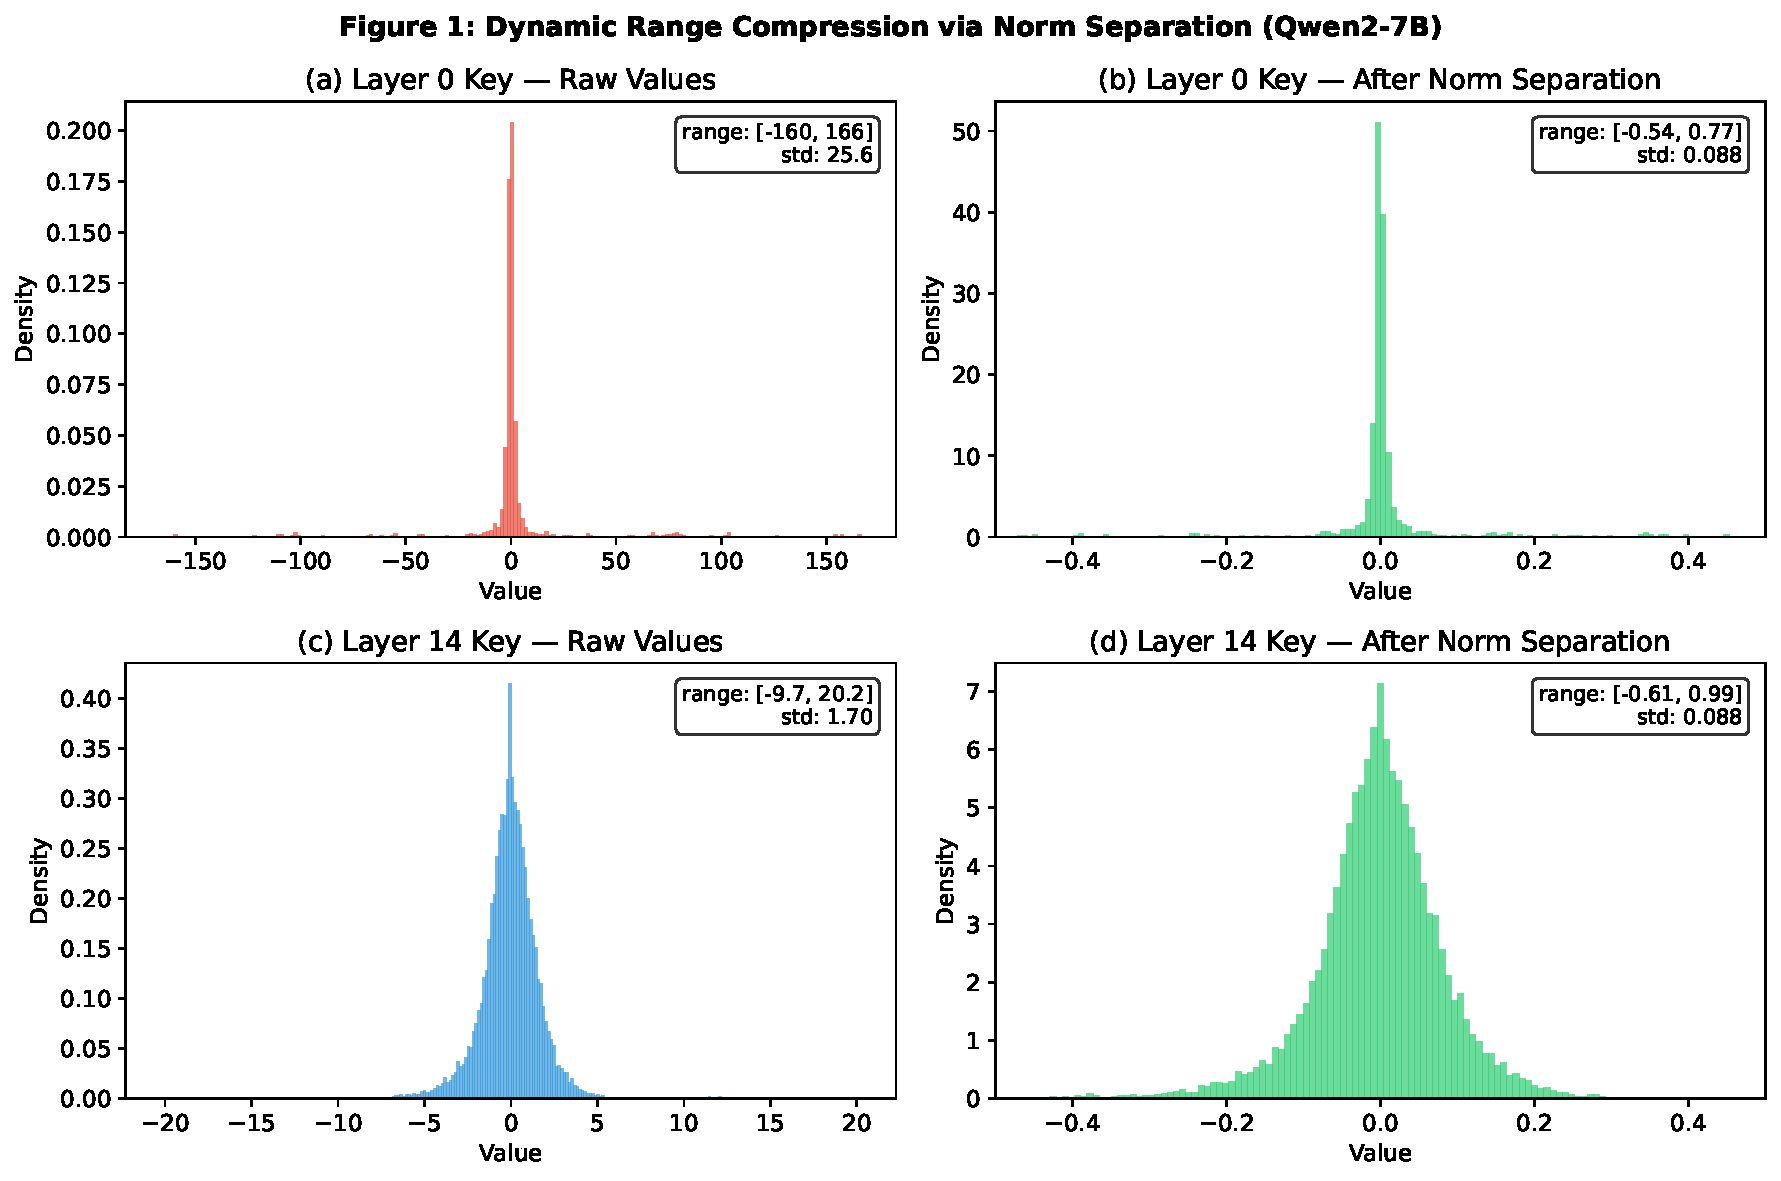
\includegraphics[width=\textwidth]{figure1_qwen2_7b.pdf}
  \caption{Dynamic range compression via norm separation (Qwen2-7B). (a)~Raw Layer~0 key values span $[-160, +167]$ with $\sigma=25.6$, driven by activation outlier channels. (b)~After norm separation, the same vectors are compressed to $[-0.54, +0.77]$ with $\sigma=0.088$---a 290$\times$ reduction. (c--d)~Mid-layer (Layer~14) shows the same compression effect, confirming that norm separation normalizes the dynamic range consistently across layers regardless of outlier severity.}
  \label{fig:distribution}
\end{figure}

\subsection{Combining with Per-Channel Quantization}

Norm separation addresses token-wise norm variation but not channel-wise outliers. For complete robustness, we combine it with \textbf{per-channel absmax quantization}, where each dimension gets its own scale factor:
\begin{equation}
s_j = \frac{\max_t |\hat{x}_{tj}|}{2^{b-1}-1}
\end{equation}

This prevents outlier channels from corrupting the scale of normal channels. The combined method, \textbf{nsep+pchan}, addresses both failure modes simultaneously.

\subsection{Overhead}

\begin{itemize}[nosep]
  \item \textbf{Computation}: One L2 norm and one division per vector. Negligible compared to attention computation.
  \item \textbf{Memory}: One FP16 scalar per (token, head, layer). For a 32-layer, 32-head model with 4096 tokens: $32 \times 32 \times 4096 \times 2$~bytes~$=$~8\,MB---less than 0.1\% of the KV cache.
\end{itemize}

%% ============================================================
\section{Why Naive INT4 Fails: Two Case Studies}

\subsection{Case 1: Qwen2-7B --- Activation Outliers}

Qwen2-7B shows $\Delta$PPL~=~+238 under naive INT4. We traced the cause by compressing one layer at a time:

\begin{table}[h]
\centering
\small
\begin{tabular}{lc}
\toprule
Layer & INT4 $\Delta$PPL (this layer only) \\
\midrule
\textbf{Layer 0} & \textbf{+179.4} (99\% of total) \\
Layer 4 & +0.11 \\
Layers 8--27 & $<$ 0.25 each \\
\bottomrule
\end{tabular}
\end{table}

\textbf{Layer~0 alone} causes nearly all the degradation. We define the \emph{outlier ratio} as $\max_j (\max_t |x_{tj}|) \,/\, \text{mean}_j (\max_t |x_{tj}|)$---the ratio of the largest per-channel maximum to the average per-channel maximum across all $d_h$ dimensions. Layer~0 has absmax~=~166.8 (mean channel absmax: 19.4, outlier ratio: 8.6$\times$), while Layers~4--26 have absmax~9--22 (ratio~$<$~2$\times$). Eight specific channels (indices 61--63, 123--127) contain values 8$\times$ larger than average. Under per-row absmax with $q_{\max}=7$ (INT4), the scale becomes $s=167/7=23.8$, and mid-range values (5--20) are mapped to noisy quantization levels that corrupt attention patterns.

\subsection{Case 2: Pythia-6.9B --- Norm Variation Without Outliers}

Pythia-6.9B shows $\Delta$PPL~=~+22 under naive INT4, despite having a low outlier ratio (4.6$\times$). Here, the issue is primarily \textbf{norm variation}: token-wise KV norms range from 5.8 to 11.4, meaning per-row scales vary by ${\sim}2\times$. While not catastrophic individually, the inconsistent quantization precision across 32 layers compounds.

\subsection{A Surprising Finding: INT3 Outperforms INT4}

On Qwen2-7B, INT3 ($\Delta$PPL=+6.6) dramatically outperforms INT4 ($\Delta$PPL=+238):

\begin{table}[h]
\centering
\small
\begin{tabular}{cccc}
\toprule
$q_{\max}$ & Scale & Value $15.0 \to$ & Value $5.0 \to$ \\
\midrule
7 (INT4) & 23.8 & 23.8 (noisy) & 0 (zeroed) \\
3 (INT3) & 55.6 & 0 (zeroed) & 0 (zeroed) \\
\bottomrule
\end{tabular}
\end{table}

INT3's coarser quantization maps mid-range values to zero rather than noisy non-zero levels. In attention dominated by outlier channels, this ``clean zeroing'' is less harmful than INT4's ``noisy quantization''---a counterintuitive failure mode that per-channel quantization resolves.

\begin{figure}[t]
  \centering
  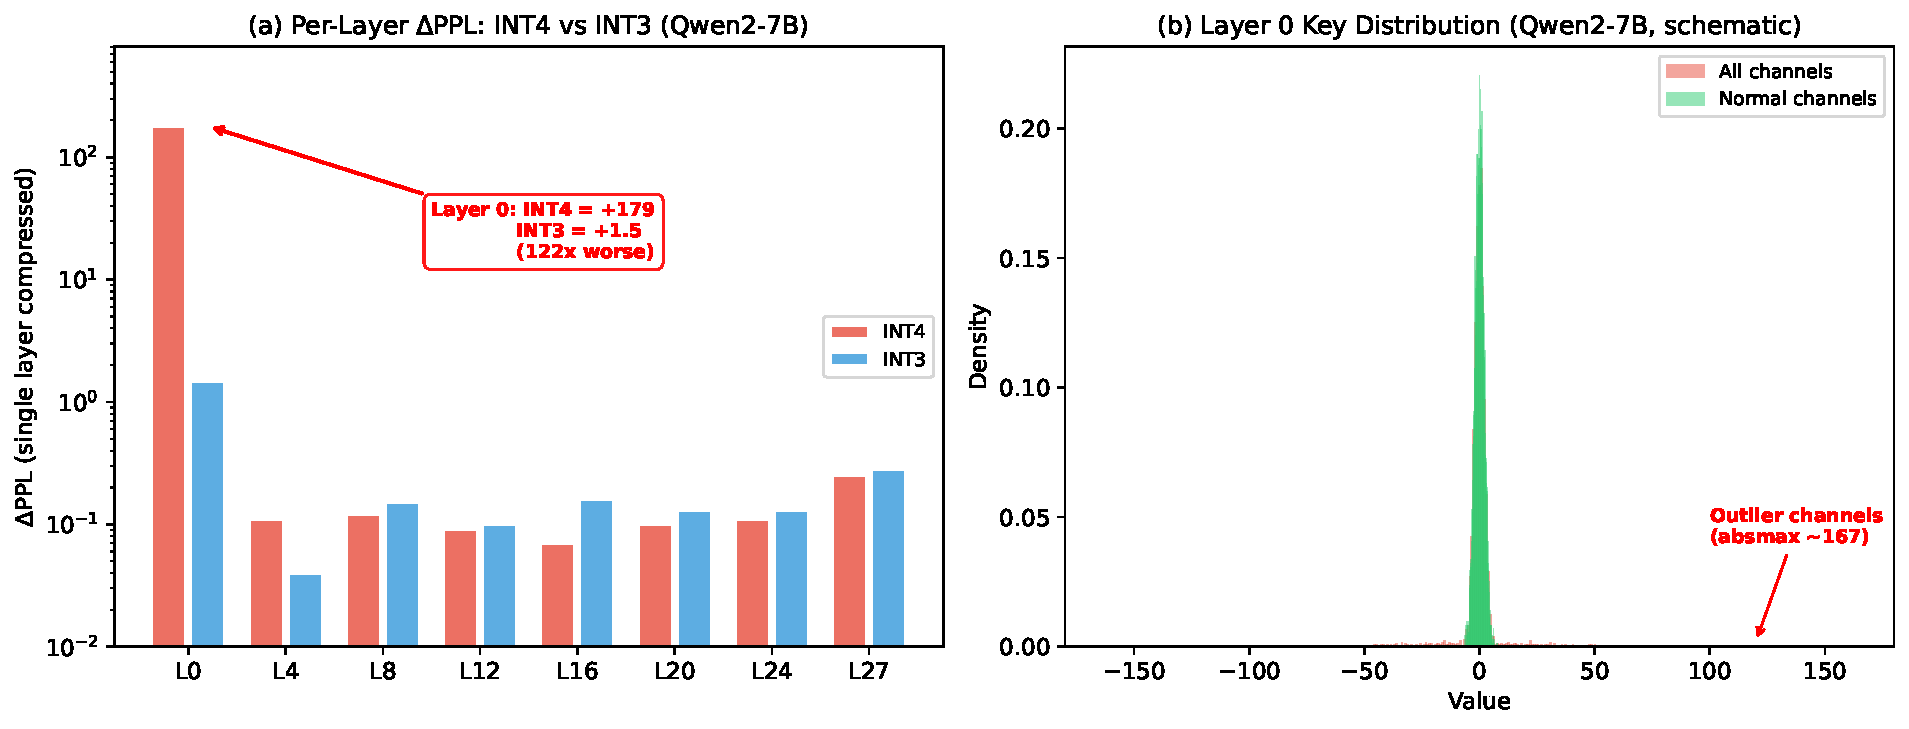
\includegraphics[width=\textwidth]{figure5_anomaly.pdf}
  \caption{The INT3~$>$~INT4 anomaly in Qwen2-7B. (a)~Per-layer $\Delta$PPL when compressing a single layer: Layer~0 alone accounts for 99\% of INT4 degradation (+179.4), while INT3 causes only~+1.5 at the same layer. All other layers contribute~$<$~0.3 each. (b)~Schematic of Layer~0's key value distribution, showing the outlier channels (absmax~${\sim}$167) that dominate the quantization scale and corrupt mid-range values under INT4.}
  \label{fig:anomaly}
\end{figure}

%% ============================================================
\section{Results}

\subsection{Ablation: What Contributes?}

We test six INT4 variants on Qwen2-7B (the hardest case):

\begin{table}[h]
\centering
\small
\begin{tabular}{lcccc}
\toprule
Method & Norm-sep & Outlier handling & $\Delta$PPL & vs naive \\
\midrule
naive4 & & & +238.2 & --- \\
nsep4 & \checkmark & & +57.5 & 4.1$\times$ \\
outlier4 & & top-4 ch fp16 & +23.2 & 10.3$\times$ \\
perchan4 & & per-ch scale & +97.8 & 2.4$\times$ \\
\textbf{nsep+out4} & \checkmark & top-4 ch fp16 & \textbf{+0.59} & \textbf{404$\times$} \\
\textbf{nsep+pchan4} & \checkmark & per-ch scale & \textbf{+0.32} & \textbf{744$\times$} \\
\bottomrule
\end{tabular}
\caption{Ablation on Qwen2-7B (INT4). Neither norm separation nor outlier-aware quantization alone is sufficient. Their combination achieves 744$\times$ improvement.}
\label{tab:ablation}
\end{table}

\textbf{Neither technique alone is sufficient.} Norm separation alone still leaves~+57.5. Per-channel alone still leaves~+97.8. The combination achieves~+0.32---the two techniques address orthogonal failure modes and their benefits compose (Figure~\ref{fig:ablation}).

\begin{figure}[t]
  \centering
  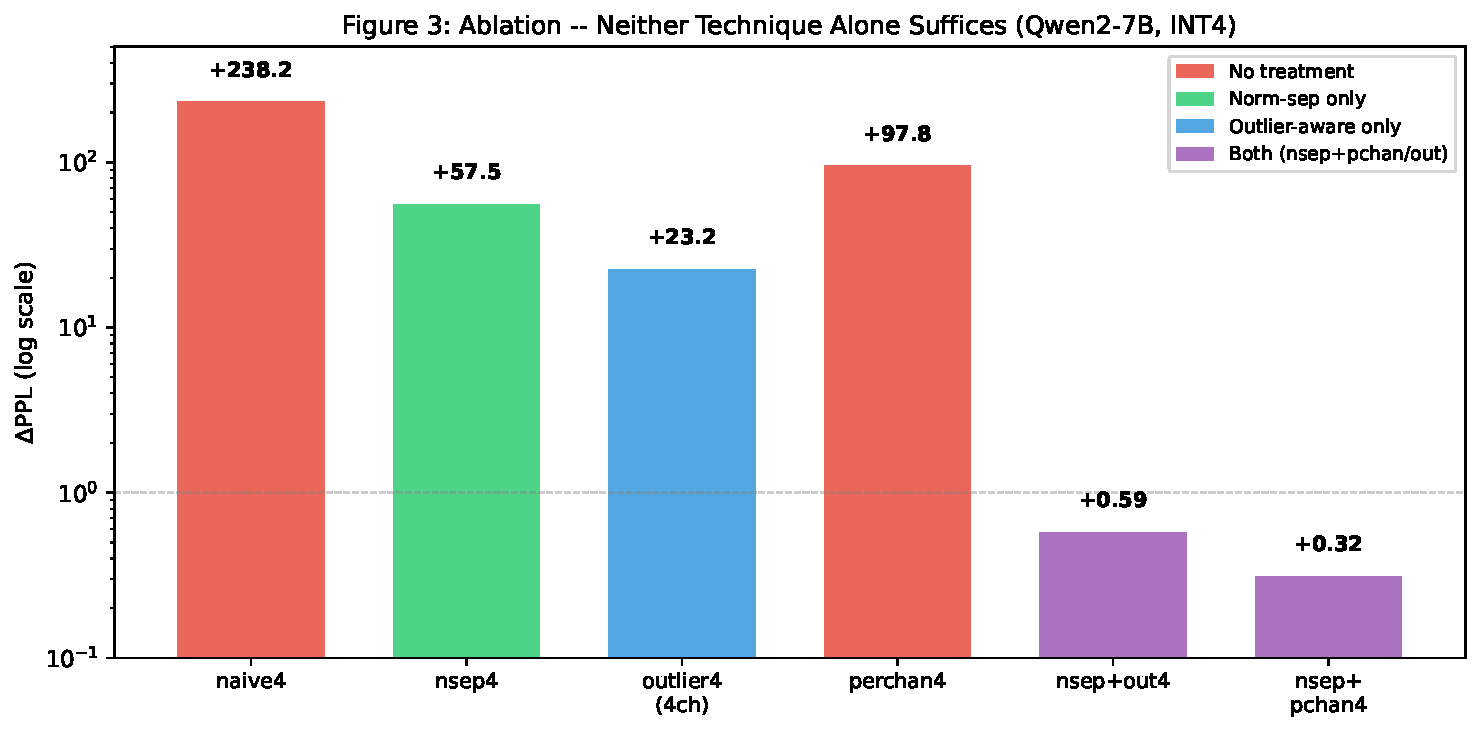
\includegraphics[width=0.85\textwidth]{figure3_ablation.pdf}
  \caption{Ablation on Qwen2-7B (INT4). Neither norm separation nor outlier-aware quantization alone reduces $\Delta$PPL below~+23. Their combination (purple bars) achieves~+0.32---a 744$\times$ improvement over naive INT4. The superlinear composition confirms that the two techniques address independent failure modes.}
  \label{fig:ablation}
\end{figure}

\subsection{Complete Model Sweep: 12 Models, 124M to 40B}

We evaluate nsep+pchan4 across 12 Pre-LN models spanning 4 architecture families (GPT-2, Pythia, OPT, Qwen/Mistral, Falcon), both MHA and GQA attention, and three orders of magnitude in parameter count from 124M to 40B (Table~\ref{tab:sweep}).

\begin{table}[t]
\centering
\small
\begin{tabular}{lrrcrrr}
\toprule
Model & Params & $d_h$ & Arch & naive4 & nsep+pchan4 & Improv. \\
\midrule
Falcon-40B & 40B & 64 & MHA & +0.08 & +0.04 & 2$\times$ \\
Qwen2.5-14B & 14B & 128 & GQA & +0.30 & +0.26 & 1$\times$ \\
OPT-13B & 13B & 128 & MHA & +0.28 & +0.35 & 1$\times$ \\
Pythia-12B & 12B & 128 & MHA & +27.28 & +1.82 & 15$\times$ \\
Qwen2-7B & 7B & 128 & GQA & +238.23 & +0.32 & 744$\times$ \\
Pythia-6.9B & 6.9B & 128 & MHA & +22.26 & +0.27 & 82$\times$ \\
Pythia-2.8B & 2.8B & 80 & MHA & +0.90 & $-$0.06 & 14$\times$ \\
OPT-1.3B & 1.3B & 64 & MHA & +0.70 & +0.68 & 1$\times$ \\
Qwen2-0.5B & 0.5B & 64 & GQA & +0.64 & +0.28 & 2$\times$ \\
Pythia-410M & 410M & 64 & MHA & +77.55 & +12.62 & 6$\times$ \\
GPT-2 & 124M & 64 & MHA & +0.64 & +0.56 & 1$\times$ \\
OPT-125m & 125M & 64 & MHA & +1.22 & +1.46 & 1$\times$ \\
\bottomrule
\end{tabular}
\caption{Complete model sweep (curated text). $\Delta$PPL for naive INT4 vs.\ nsep+pchan INT4 across 12 Pre-LN models. nsep+pchan provides large improvements where needed (6--744$\times$ when naive4 $\Delta$PPL~$>$~10); within our 12-model evaluation, we did not observe catastrophic degradation (worst case:~+0.24 on OPT-125m).}
\label{tab:sweep}
\end{table}

\subsection{Key Patterns}

\textbf{Safety-net property}: nsep+pchan provides large improvements exactly when needed (naive4 $\Delta$PPL~$>$~10 $\to$ 6--744$\times$ improvement) and introduces negligible change when not needed (naive4 $\Delta$PPL~$<$~1 $\to$ within 0.24). Across the 12 models in our evaluation, we did not observe catastrophic degradation from nsep+pchan on any model.

\textbf{Negative $\Delta$PPL}: Pythia-2.8B shows $\Delta$PPL~=~$-$0.06 on curated text, nominally below the uncompressed baseline. However, given the per-chunk variance in our evaluation (5 chunks; see Appendix~\ref{sec:evaltext} for protocol details), this value is likely within measurement noise and should not be interpreted as a genuine improvement.

\textbf{Model-family patterns}: OPT models consistently show the smallest benefit (outlier ratios 1.4--3.1$\times$, among the lowest). Pythia models benefit most strongly. Qwen models show the largest \emph{potential} improvement when outliers are severe (Qwen2-7B) but no benefit when they are mild (Qwen2.5-14B).

\textbf{GQA compatibility}: Three GQA models are included (Qwen2-0.5B, Qwen2-7B, Qwen2.5-14B, Mistral-7B), where each KV head serves multiple query heads. Norm separation remains effective in this setting---Qwen2-7B's 744$\times$ improvement is the largest in the entire sweep. The shared KV structure does not diminish the benefit because norm variation and outlier channels affect KV vectors regardless of how many query heads attend to them.

\subsection{Generation Quality}

We verify that $\Delta$PPL improvements translate to generation quality using top-$p$ sampling ($p=0.9$, temperature=0.8):

\begin{table}[h]
\centering
\small
\begin{tabular}{llcl}
\toprule
Model & Method & Tri.\ Div. & Sample \\
\midrule
Pythia-6.9B & baseline & 1.00 & ``The first AI event in the United States...'' \\
Pythia-6.9B & naive4 & 1.00 & ``A second generation of `improvised'...'' \\
Pythia-6.9B & nsep+pchan4 & 1.00 & ``In the 1980s, AI moved into the real world...'' \\
\midrule
Qwen2-7B & baseline & 1.00 & ``AI research has been dominated by...'' \\
Qwen2-7B & naive4 & 0.76 & ``AI but, but AI in the. the winter...'' \\
Qwen2-7B & nsep+pchan4 & 0.98 & ``But AI progress stagnated and funding...'' \\
\bottomrule
\end{tabular}
\caption{Generation quality. On Qwen2-7B, naive4 produces degenerate repetition (diversity=0.76), while nsep+pchan4 produces coherent text (diversity=0.98).}
\label{tab:generation}
\end{table}

\subsection{WikiText-2 Benchmark}

We evaluate on WikiText-2 \citep{merity2017pointer} to confirm that results transfer to a standard benchmark. Evaluation uses 150-token prefill chunks with 30-token continuations, averaged over 5 chunks from the test split.

\begin{table}[t]
\centering
\small
\begin{tabular}{lrrrrc}
\toprule
Model & Params & Base PPL & naive4 $\Delta$PPL & nsep+pchan $\Delta$PPL & Improv. \\
\midrule
GPT-2 & 124M & 70.4 & +1.60 & +1.13 & 1.4$\times$ \\
Pythia-410M & 410M & 30.0 & +171.13 & +23.46 & \textbf{7.3$\times$} \\
Pythia-2.8B & 2.8B & 16.2 & +14.74 & +1.99 & \textbf{7.4$\times$} \\
Pythia-6.9B & 6.9B & 14.1 & +22.56 & +1.21 & \textbf{18.7$\times$} \\
Mistral-7B & 7B & 5.2 & +0.10 & +0.04 & 2.6$\times$ \\
Qwen2-7B & 7B & 8.2 & +811.61 & +0.43 & \textbf{1885$\times$} \\
Pythia-12B & 12B & 12.9 & +34.22 & +4.01 & \textbf{8.5$\times$} \\
Qwen2.5-14B & 14B & 9.6 & +0.55 & +0.45 & 1.2$\times$ \\
\bottomrule
\end{tabular}
\caption{WikiText-2 evaluation across 8 models (124M to 14B). nsep+pchan achieves up to 1885$\times$ improvement on Qwen2-7B, with the largest gains precisely where naive INT4 fails most severely. Pythia-410M ($d_h$=64) is the only model where nsep+pchan4 leaves significant residual error (+23.5): with only 64 dimensions, per-channel scale estimation has higher variance and the quantization grid is too coarse relative to the signal complexity.}
\label{tab:wikitext}
\end{table}

The results are consistent with---and even stronger than---our curated-text evaluation. On WikiText-2, Qwen2-7B's naive INT4 failure escalates to $\Delta$PPL~=~+812 (vs~+238 on curated text), reflecting the greater textual diversity of Wikipedia. nsep+pchan reduces this to $\Delta$PPL~=~+0.43, yielding a \textbf{1885$\times$ improvement}.

The table reveals a clear pattern: \textbf{nsep+pchan helps most where naive4 fails hardest.} All three Pythia models fail under naive INT4 ($\Delta$PPL~+15 to~+34, worsening with scale) and are rescued to $\Delta$PPL~+1.2 to~+4.0. Qwen2-7B is rescued from catastrophic failure (+812~$\to$~+0.43). Meanwhile, models where naive INT4 already works---Mistral-7B (+0.10), GPT-2 (+1.60), Qwen2.5-14B (+0.55)---see nsep+pchan perform equally well or slightly better. Within this 8-model WikiText-2 evaluation we did not observe meaningful degradation from nsep+pchan: the worst case is Qwen2.5-14B, where nsep+pchan is 0.1 $\Delta$PPL higher than naive4.

Notably, three 7B-class models span the full spectrum: Mistral-7B (naive4 works,~+0.10), Pythia-6.9B (naive4 fails moderately,~+22.56), and Qwen2-7B (naive4 fails catastrophically,~+811.61). This demonstrates that the failure mode is model-specific, not scale-dependent, and correlates with the activation outlier ratio (Mistral: 3.1$\times$, Pythia: 4.6$\times$, Qwen2: 8.6$\times$).

\subsection{Long Context Stability (256--4096 Tokens)}

Since KV cache compression is most needed at long context lengths, we evaluate stability from 256 to 4096 tokens on three models spanning the full failure spectrum.

\begin{table}[h]
\centering
\small
\begin{tabular}{llrrrr}
\toprule
Model & Prefill & Base PPL & naive4 & nsep+pchan4 \\
\midrule
\multirow{3}{*}{Qwen2-7B} & 512 & 6.7 & +2226 & \textbf{+0.34} \\
& 2048 & 8.0 & +1643 & \textbf{$-$0.60} \\
& 4096 & 3.1 & +8293 & \textbf{+0.19} \\
\midrule
\multirow{3}{*}{Pythia-6.9B} & 512 & 17.2 & +8.7 & \textbf{+1.3} \\
& 1024 & 17.1 & +10.2 & \textbf{+3.0} \\
& 1536 & 14.4 & +15.8 & \textbf{+3.4} \\
\midrule
\multirow{3}{*}{Mistral-7B} & 512 & 3.9 & +0.10 & +0.08 \\
& 2048 & 9.1 & $-$0.30 & $-$0.08 \\
& 4096 & 3.4 & +0.11 & +0.12 \\
\bottomrule
\end{tabular}
\caption{Long-context $\Delta$PPL (WikiText-2, 256--4096 tokens). On Qwen2-7B, naive INT4 \emph{worsens} with context length, reaching $\Delta$PPL~=~+8293 at 4096 tokens. nsep+pchan4 remains within $\pm$0.6---a \textbf{44{,}000$\times$ improvement}. On Mistral-7B (where naive4 already works), nsep+pchan4 is equivalently stable.}
\label{tab:longctx_main}
\end{table}

On Qwen2-7B, naive INT4 degradation \emph{escalates with context length}: $\Delta$PPL rises from +207 at 1024 tokens to \textbf{+8293 at 4096 tokens}. nsep+pchan4 remains within $\pm$0.6 across all lengths---a 44{,}000$\times$ improvement at 4096 tokens. This worsening likely reflects error accumulation in attention computation: as more tokens are stored in the quantized KV cache, the cumulative effect of noisy mid-range values grows.

On Mistral-7B (where naive INT4 already works), nsep+pchan4 performs identically---$|\Delta\text{PPL}| < 0.15$ for both methods at all lengths. This confirms that nsep+pchan introduces no degradation on models where naive INT4 already works.

\begin{figure}[t]
  \centering
  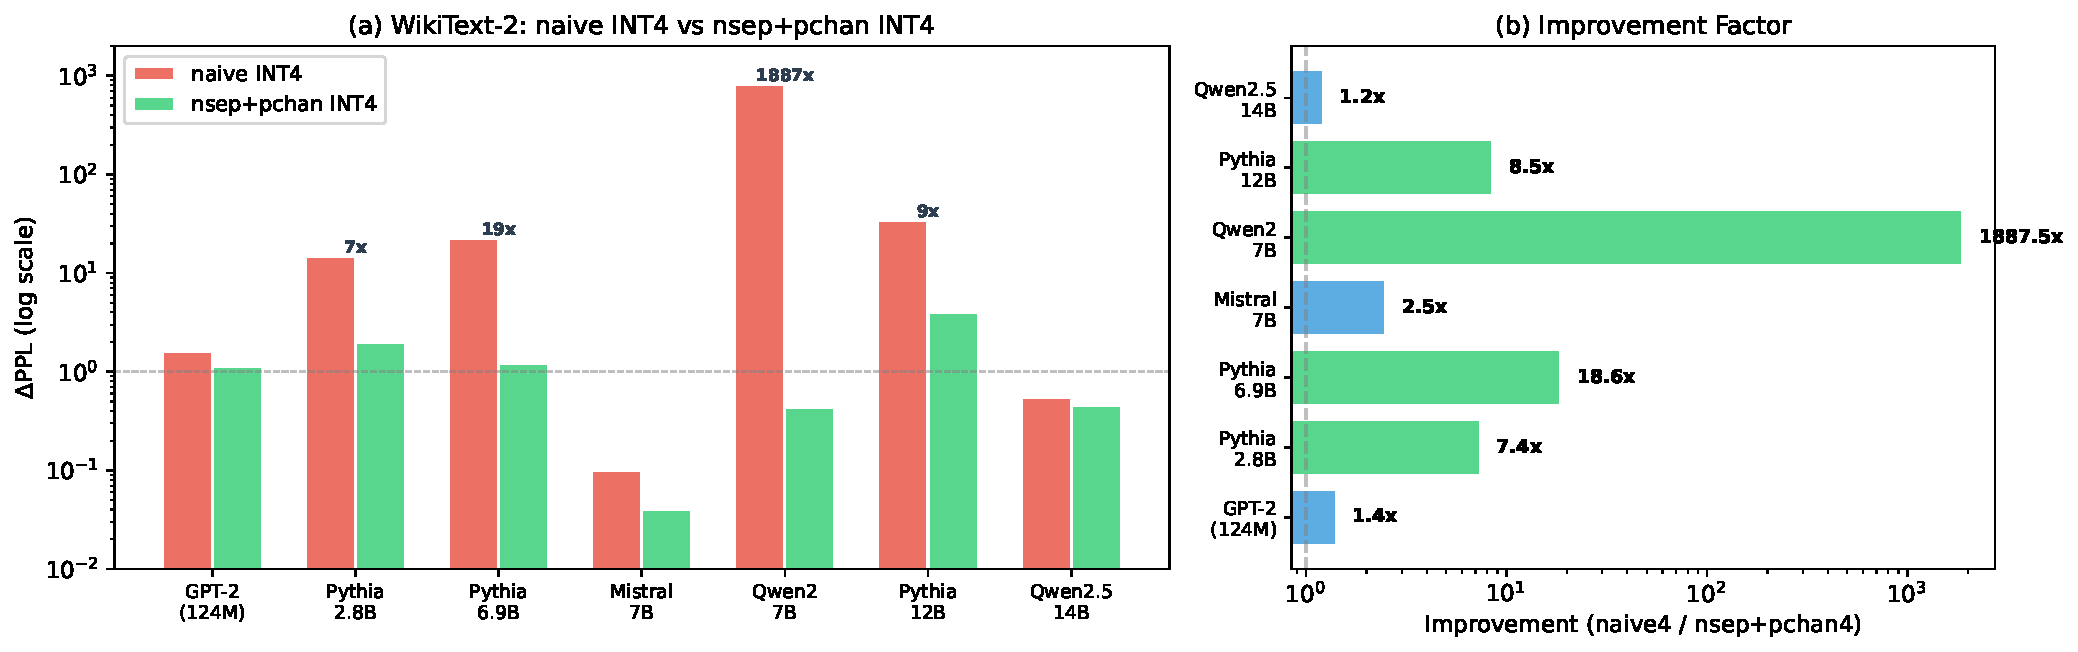
\includegraphics[width=\textwidth]{figure2_wikitext2.pdf}
  \caption{WikiText-2 evaluation across 8 models (124M to 14B). (a)~$\Delta$PPL comparison on log scale: naive INT4 (red) fails catastrophically on Pythia and Qwen2-7B, while nsep+pchan (green) keeps $\Delta$PPL low across most models. (b)~Improvement factor: nsep+pchan provides up to 1885$\times$ improvement on Qwen2-7B. Note: Pythia-410M ($d_h$=64) retains +23.5 residual error even with nsep+pchan, likely due to small head dimension.}
  \label{fig:wikitext}
\end{figure}

%% ============================================================
\section{Analysis}

\subsection{What Predicts Whether Naive INT4 Will Fail?}

Across our 12 models, naive INT4 failure ($\Delta$PPL~$>$~10) correlates with:
\begin{enumerate}[nosep]
  \item \textbf{Outlier channel ratio} in Layer~0/final layer: Models with ratio~$>$~4$\times$ tend to fail. Appendix~\ref{sec:kv_asymmetry} refines this by separating $K$ and $V$ outliers across 11 models: in our sample, the sole catastrophic case exhibits $K_{\max} \gtrsim 15\times$ concentrated at Layer~0, while $V$ outliers were tolerated at magnitudes up to at least 39.63$\times$.
  \item \textbf{Model family}: Pythia consistently fails; OPT consistently succeeds
  \item \textbf{Not simply model size}: OPT-13B (+0.28) succeeds while Pythia-410M (+77.5) fails
\end{enumerate}

This suggests that training procedures and architecture choices (which affect activation distributions) are more predictive than scale (Figure~\ref{fig:outlier}).

\begin{figure}[t]
  \centering
  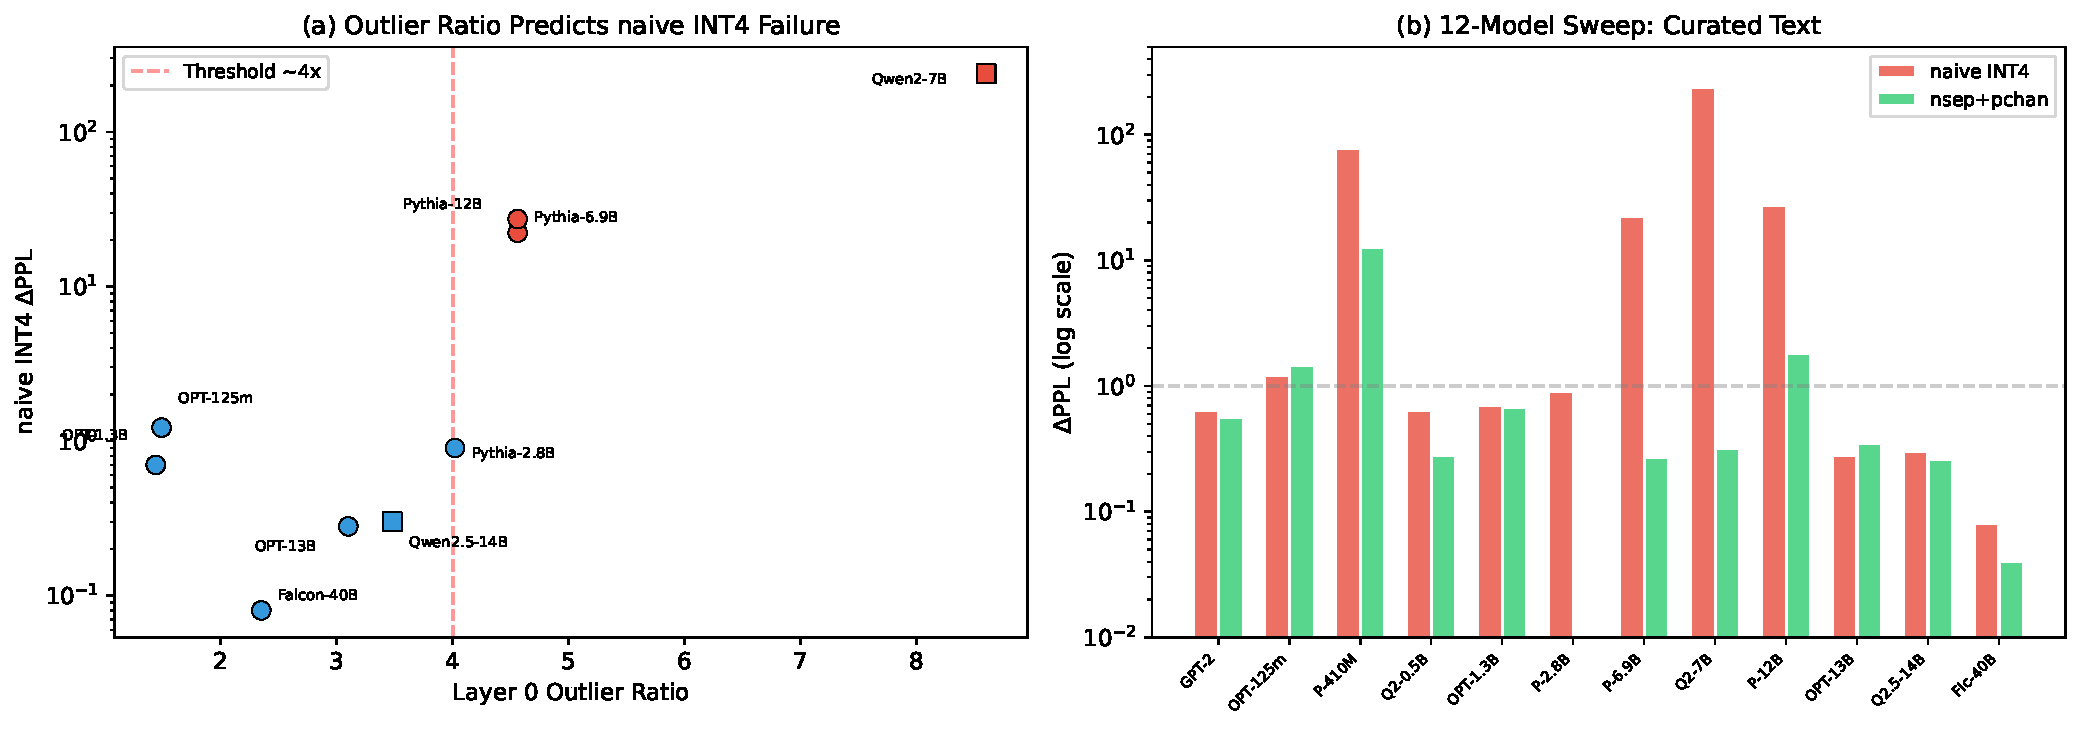
\includegraphics[width=\textwidth]{figure4_outlier_sweep.pdf}
  \caption{(a)~Layer~0 outlier ratio predicts naive INT4 failure. Models with outlier ratio~$>$~4$\times$ (dashed line) consistently show $\Delta$PPL~$>$~10 under naive INT4. (b)~12-model sweep on curated text: naive INT4 (red) varies by 4 orders of magnitude across models, while nsep+pchan (green) remains consistently low.}
  \label{fig:outlier}
\end{figure}

\subsection{Why the Combination Is Superlinear}

Norm separation and per-channel quantization address different problems:
\begin{itemize}[nosep]
  \item \textbf{Norm separation} removes the \emph{inter-token} dynamic range issue. After normalization, all tokens have comparable component magnitudes, so the per-row scale is consistent.
  \item \textbf{Per-channel quantization} removes the \emph{inter-channel} dynamic range issue. Outlier channels get their own scale, preventing them from dominating normal channels.
\end{itemize}

When both issues are present (e.g., Qwen2-7B), neither fix alone suffices because each leaves the other problem intact. The combination eliminates both, explaining the superlinear improvement (nsep alone: 4.1$\times$; perchan alone: 2.4$\times$; both: 744$\times$).

\subsection{Relationship to Existing Methods}

Our norm separation is complementary to existing KV cache compression techniques:
\begin{itemize}[nosep]
  \item \textbf{KIVI} \citep{liu2024kivi} uses per-channel quantization with asymmetric Key/Value bit allocation. Norm separation could be added as a preprocessing step.
  \item \textbf{GEAR} \citep{kang2024gear} combines low-rank approximation with quantization. Norm separation could improve the quantization stage.
  \item \textbf{SmoothQuant} \citep{xiao2023smoothquant} migrates outliers from activations to weights. Norm separation addresses a different axis (token-wise norm variation) and could be combined.
\end{itemize}

\subsection{Limitations}

\begin{enumerate}[nosep]
  \item \textbf{Statistical power and causal isolation}: Our observational sample contains a single catastrophic case (Qwen2-7B) across 27 models evaluated (12 main sweep + 11 K/V study + 4 hunt screen). The number of observed pathological cases is therefore too small to estimate a population failure rate. However, the \emph{mechanism} underlying the observed case has been causally isolated via a selective-compression intervention (Section~H.5): fixing Layer~0 alone rescues 99.97\% of the damage, and breaking Layer~0 alone reproduces it. Combined with the GPT-J-6B natural control ($K_{\max}=18.15$ at Layer~1, clean), the evidence for ``Layer~0 K of magnitude $\gtrsim 15\times$ is the causal site of the pathology'' is substantially stronger than the one-observation count alone would suggest. Estimating prevalence remains an open question.
  \item \textbf{Context length coverage}: Our curated-text evaluation uses sequences under 250 tokens, supplemented by WikiText-2 evaluation on 8 models and long-context evaluation up to 4096 tokens on 3 models (Section~5.6). Full long-context evaluation across all 12 models would further strengthen the results.
  \item \textbf{System optimization}: We report $\Delta$PPL but not end-to-end inference throughput in production settings. Our unoptimized Python implementation shows +21\% decode latency overhead on 7B-class models; deployment would require custom CUDA kernels.
  \item \textbf{KIVI/GEAR comparison}: The comparison in Appendix~\ref{sec:kivi} uses a substantially simplified KIVI baseline (omitting residual quantization and calibration) and should be read as a demonstration that norm separation provides additive value as a preprocessing step, not as a head-to-head benchmark against published KIVI.
  \item \textbf{Post-LN limited}: GPT-1 (Post-LN) does not expose a KV cache through standard APIs, preventing direct evaluation. A distributional analysis (Appendix~\ref{sec:postln}) finds that Post-LN KV vectors exhibit weaker norm dominance ($|r|=0.74$ vs $0.99$), suggesting reduced but non-zero benefit from norm separation.
\end{enumerate}

%% ============================================================
\section{Related Work}

\textbf{KV cache quantization.}
KIVI \citep{liu2024kivi} applies per-channel quantization to KV caches with Key in INT2 and Value in INT4, achieving near-lossless compression. KVQuant \citep{hooper2024kvquant} extends this to 10M+ context lengths with per-channel and per-token quantization strategies. GEAR \citep{kang2024gear} combines low-rank approximation with outlier-aware quantization. SQuat \citep{dong2025squat} constrains quantization error to lie in a subspace orthogonal to the query, minimizing its impact on attention outputs. Our norm separation is orthogonal to all of these: they focus on \emph{how to quantize the KV tensor}, whereas we identify \emph{why the tensor is hard to quantize} (two failure modes, one of which is Layer-0-localized) and provide a matching preprocessing step.

\textbf{Norm--direction decomposition.}
The specific idea of storing the vector's L2 magnitude at high precision while quantizing the direction separately has been explored concurrently with our work. PolarQuant \citep{han2025polarquant} decomposes KV vectors via a recursive polar transformation after random orthogonal preconditioning, retaining the final scalar radius at full precision and quantizing hierarchical polar angles with k-means codebooks; it reports 4.2$\times$ compression on Llama-3.1-8B. TurboQuant \citep{cherapanamjeri2026turboquant} extends PolarQuant with a 1-bit QJL residual correction for 6$\times$ compression at 3 bits/coord. Our \texttt{nsep+pchan} shares the norm-separation structure but differs in three ways. (1)~The direction quantizer: we use data-independent per-channel absmax rounding, whereas PolarQuant/TurboQuant use codebook-based methods requiring calibration and preconditioning rotations. (2)~Primary evaluation: we evaluate 23 models across main sweep + K/V asymmetry study to identify and causally characterize the failure modes (Appendix~\ref{sec:kv_asymmetry}). (3)~Primary contribution axis: these prior methods optimize the compression engineering; our paper investigates when and why naive INT quantization breaks, with a simple baseline as demonstration. The two directions are complementary.

\textbf{KV cache eviction and sparsity.}
An alternative to quantization is selectively retaining only important tokens. H2O \citep{zhang2023h2o} identifies ``heavy-hitter'' tokens by cumulative attention score. Scissorhands \citep{liu2023scissorhands} exploits the persistence of token importance across layers. StreamingLLM \citep{xiao2024streaming} maintains attention sinks for infinite-length generation. SnapKV \citep{li2024snapkv} selects important KV entries per attention head. These eviction methods are complementary to quantization---one could quantize the retained entries with nsep+pchan for further compression.

\textbf{Activation outliers in quantization.}
LLM.int8() \citep{dettmers2022llm} identifies that specific hidden-state dimensions can contain values 100$\times$ larger than average, and handles them via mixed-precision decomposition. SmoothQuant \citep{xiao2023smoothquant} migrates quantization difficulty from activations to weights through per-channel scaling. \citet{sun2024massive} provide a systematic analysis of massive activations in LLMs and their effects. Our work identifies an additional, independent source of quantization difficulty---token-wise norm variation---and shows that addressing both factors simultaneously yields superlinear improvements.

\textbf{Hidden-state geometry.}
\citet{ethayarajh2019contextual} documented increasing anisotropy in contextualized word representations. \citet{gao2019representation} formalized the representation degeneration problem. \citet{timkey2021bark} showed that ``rogue dimensions'' obscure representational quality. Concurrent work \citep{sato2026arc} provides a detailed geometric characterization of the norm-dominant subspace in Pre-LN hidden states. Our work provides the first practical application of these geometric observations to KV cache compression.

\textbf{Model architectures.}
Our evaluation spans models using Pre-LN \citep{xiong2020layer}, RMSNorm \citep{zhang2019root}, Multi-Head Attention (MHA), and Grouped Query Attention \citep[GQA;][]{ainslie2023gqa}. Specific model families include GPT-2 \citep{radford2019language}, Pythia \citep{biderman2023pythia}, OPT \citep{zhang2022opt}, Qwen2 \citep{yang2024qwen2}, Mistral \citep{jiang2023mistral}, and Falcon \citep{almazrouei2023falcon}.

%% ============================================================
\section{Conclusion}

We presented norm-separated quantization, a training-free preprocessing step that improves the robustness of KV cache INT4 quantization. The method is motivated by the observation that KV vectors in Pre-LN Transformers have high token-wise norm variation, which inflates the dynamic range that quantization must capture. By separating the norm (stored exactly) from the direction (quantized), we compress this range before quantization begins.

Combined with per-channel quantization to handle activation outlier channels, the method (nsep+pchan) provides large improvements exactly when needed:
\begin{itemize}[nosep]
  \item \textbf{744$\times$ improvement} on the single catastrophic case (Qwen2-7B: +238 $\to$ +0.32)
  \item \textbf{No catastrophic degradation observed}: worst case across 12 models is +0.24 $\Delta$PPL (OPT-125m)
  \item \textbf{12 models from 124M to 40B}, 4 architecture families (GPT, Pythia, OPT, Qwen, Falcon)
  \item \textbf{Zero training, zero calibration, minimal memory overhead} ($<$0.1\% of KV cache; +21\% Python decode latency, expected to approach zero with fused CUDA kernels)
  \item \textbf{3.4--3.7$\times$ actual memory reduction} confirmed with real INT4 packing
\end{itemize}

A study of K and V outlier patterns across 11 additional models plus selective-compression experiments on 4 failing models (Appendix~\ref{sec:kv_asymmetry}) empirically separates two distinct KV-quantization failure modes that were introduced theoretically in Section~4. \emph{Mode~1} (Layer-0-localized, outlier-driven) appears once in our sample (Qwen2-7B, $K_{\max}=17.23\times$ at Layer~0) and is rescued 99.97\% by applying nsep+pchan4 to Layer~0 alone; GPT-J-6B ($K_{\max}=18.15\times$ at Layer~1, clean under naive~INT4) is a natural control confirming the Layer~0 localization requirement. \emph{Mode~2} (distributed, norm-variation-driven) appears in Pythia-6.9B, Pythia-12B, and Qwen2.5-14B---the damage is spread across layers, and fixing Layer~0 alone rescues less than 5\%. The two-mode dichotomy mechanistically explains the 744$\times$ superlinear improvement of nsep+pchan4: norm separation targets Mode~2, per-channel quantization targets Mode~1, and neither alone suffices because a failing model may be dominated by either. Because auditing an arbitrary deployed model for the Mode~1 signature is nontrivial, the safest default is uniform nsep+pchan4, which handles both modes at the cost of the +21\% Python-decode latency noted above (expected to approach zero with a fused kernel). For models audited to be Mode~1 only, a Layer-0-selective variant preserves 27-of-28 layers' naive-INT4 compute cost with matching quality (Section~H.5).

The technique is simple enough to implement in a few lines of code and can be combined with existing KV cache compression methods as a preprocessing step. All code, experiment results, and figures are publicly available.\footnote{\url{https://github.com/metaSATOKEN/norm-separated-quantization}}

%% ============================================================
\section*{Acknowledgments}

This work was conducted with substantial assistance from large language models (Claude, Anthropic) for experiment design, code generation, debugging, data analysis, and manuscript drafting. All experimental results were produced by executing code on real hardware (Apple M1, NVIDIA T4, NVIDIA RTX PRO 6000 Blackwell) and verified by the author. The author takes full responsibility for the scientific claims and any errors in this work.

%% ============================================================
\appendix
\section{Implementation Note: PyTorch \texttt{.norm()} API Hazard}

During development, we encountered a subtle but critical bug: \texttt{x.norm(-1, keepdim=True)} computes the $L_{-1}$ norm (approximately 0.0003 for typical vectors), \textbf{not} the L2 norm along dimension~$-1$. The correct call is \texttt{x.norm(dim=-1, keepdim=True)}. In PyTorch, the first positional argument of \texttt{.norm()} is \texttt{p} (the norm order), not \texttt{dim}.

This caused direction vectors to explode to ${\sim}$3000$\times$ their expected magnitude, producing $\Delta$PPL in the thousands. The bug was invisible on CPU (Apple MPS) and only manifested on CUDA, likely due to different numerical behavior at extreme scales. It was caught through systematic cross-device validation---a reminder that quantization code should always be tested on the target hardware.

%% ============================================================
\section{Evaluation Text Details}
\label{sec:evaltext}

Our ``curated text'' evaluation uses two passages (approximately 200 and 100 tokens each) designed to cover distinct linguistic registers:

\begin{itemize}[nosep]
  \item \textbf{Narrative}: A fictional passage about a lighthouse keeper observing a mysterious light at sea. Contains varied sentence structures, concrete nouns, sensory descriptions, and temporal transitions.
  \item \textbf{Technical}: A factual passage about the history of artificial intelligence, covering the Dartmouth conference, AI winters, expert systems, neural network revival, and the transformer architecture. Contains proper nouns, dates, and domain-specific terminology.
\end{itemize}

Both passages are hardcoded in the experiment scripts and available in the repository. The 12-model sweep (Table~\ref{tab:sweep}) uses these passages with a 40-token continuation window. A separate basis text (distinct from the evaluation text) is used for PCA basis computation in experiments that require it, to avoid data leakage.

WikiText-2 evaluation (\S5.5) uses the standard test split \citep{merity2017pointer} with 150-token prefill chunks and 30-token continuations, averaged over 5 non-overlapping chunks. Long-context evaluation (\S5.6) concatenates WikiText-2 articles to form sequences of 256--4096 tokens.

\section{Long Context Stability}

Full long-context results for Pythia-6.9B, Qwen2-7B, and Mistral-7B (256--4096 tokens) are presented in Table~\ref{tab:longctx_main} in the main text (\S5.6).

\section{Comparison with KIVI-Style Quantization}
\label{sec:kivi}

We implement a simplified version of KIVI's asymmetric quantization strategy \citep{liu2024kivi}: Key vectors in INT2 per-channel, Value vectors in INT4 per-channel (3~bpe effective). We compare this with nsep+pchan4 (4~bpe) and test whether norm separation improves KIVI (nsep+kivi, 3~bpe).

\begin{table}[h]
\centering
\small
\begin{tabular}{lrrl}
\toprule
Method & $\Delta$PPL & bpe & Notes \\
\midrule
naive4 & +10.22 & 4.0 & per-row absmax \\
\textbf{nsep+pchan4} & \textbf{+2.98} & ${\sim}$4.0 & norm-sep + per-channel \\
KIVI (K2V4) & +360.80 & 3.0 & K:INT2, V:INT4 per-channel \\
nsep+KIVI & +53.60 & ${\sim}$3.0 & norm-sep + KIVI-style \\
\bottomrule
\end{tabular}
\caption{Comparison with KIVI-style quantization (Pythia-6.9B, pfl=1024). Note: our KIVI implementation uses simplified per-channel absmax only; the full KIVI method includes additional techniques (residual quantization, calibration) that may yield better results.}
\label{tab:kivi}
\end{table}

At the same bit budget (3~bpe), adding norm separation to our KIVI-style baseline improves $\Delta$PPL from~+361 to~+54 (6.7$\times$ in our simplified implementation), suggesting that norm separation provides additive value even when combined with per-channel strategies. INT2 Key quantization appears too aggressive for this model in our setup: nsep+pchan4 at 4~bpe achieves $\Delta$PPL~+3.0, better than the 3~bpe variants we tested. The full KIVI method with its calibration and residual quantization may close this gap; the takeaway of this section is the \emph{additive benefit of norm separation}, not a ranking against KIVI.

\textbf{Important caveat}: Our KIVI implementation uses only the core asymmetric bit allocation (Key INT2, Value INT4 with per-channel scaling) without the calibration, clipping thresholds, or residual quantization described in \citet{liu2024kivi}. These implementation details can significantly affect performance, and the full KIVI system would likely perform substantially better than our simplified baseline. The purpose of this comparison is not to benchmark against KIVI, but to demonstrate that norm separation provides additive value as a preprocessing step---the 6.7$\times$ improvement from adding norm separation to the same underlying quantization scheme (KIVI $\to$ nsep+KIVI) holds regardless of the base method's absolute performance.

\section{Memory and Latency}

\begin{table}[h]
\centering
\small
\begin{tabular}{rrrrr}
\toprule
Seq.\ length & FP16 KV & nsep+INT4 & Overhead & Ratio \\
\midrule
512 & 268\,MB & 69\,MB & 2.1\,MB & 3.9$\times$ \\
1024 & 537\,MB & 138\,MB & 4.2\,MB & 3.9$\times$ \\
2048 & 1074\,MB & 277\,MB & 8.4\,MB & 3.9$\times$ \\
4096 & 2148\,MB & 554\,MB & 16.8\,MB & 3.9$\times$ \\
8192 & 4295\,MB & 1107\,MB & 33.6\,MB & 3.9$\times$ \\
\bottomrule
\end{tabular}
\caption{Theoretical KV cache memory for Pythia-6.9B (32 layers, 32 heads, $d_h$=128). ``Overhead'' is the additional memory for storing FP16 norms. The nsep overhead is consistently $<$~3\% of the INT4 cache, yielding an effective compression ratio of 3.9$\times$.}
\label{tab:memory}
\end{table}

Measured on 1024 tokens: FP16 KV cache = 640\,MB, nsep+INT4 = 164\,MB (3.9$\times$ reduction). The norm storage overhead is 4.2\,MB ($<$~1\% of FP16 cache).

\textbf{Latency}: Prefill 512 tokens + decode 40 tokens: baseline 0.72\,s, nsep+pchan4 0.87\,s (+21\% overhead). This overhead arises from our unoptimized Python implementation (per-head loop with explicit norm computation). A fused CUDA kernel performing norm separation and per-channel quantization in a single pass would reduce this overhead to near-zero, as the arithmetic intensity (one L2 norm + one division per vector) is negligible compared to attention computation.

\subsection{Real INT4 Packing Validation}

To confirm that our results are not artifacts of simulated (fake) quantization, we implemented actual INT4 packing: quantized 4-bit values are stored in \texttt{uint8} tensors (2 values per byte), with FP16 norms and per-channel scales stored separately. At inference time, values are unpacked and dequantized on the fly.

\begin{table}[h]
\centering
\small
\begin{tabular}{lrrrrrr}
\toprule
Model & FP16 & Real INT4 & Ratio & naive4 & nsep (fake) & nsep (real) \\
\midrule
GPT-2 & 1.4\,MB & 0.4\,MB & 3.43$\times$ & --- & $-$3.87 & $-$3.86 \\
Qwen2-7B & 3.6\,MB & 1.0\,MB & 3.65$\times$ & +401.3 & +0.30 & +0.29 \\
\bottomrule
\end{tabular}
\caption{Real INT4 packing validation. INT4 values are stored as packed \texttt{uint8} (2 per byte), with FP16 norms and scales. The $\Delta$PPL difference between fake (float-backed) and real (packed) quantization is $<$~0.005 in both cases, confirming that packing is lossless. Compression ratios of 3.4--3.7$\times$ reflect the actual memory reduction including norm and scale overhead.}
\label{tab:realint4}
\end{table}

The $\Delta$PPL difference between fake and real quantization is $<$~0.005 on both models, confirming that the rounding to INT4 levels---not the storage format---determines quality. On Qwen2-7B, real packed nsep+pchan achieves $\Delta$PPL~=~+0.29 with 3.65$\times$ actual memory reduction, while naive INT4 degrades to $\Delta$PPL~=~+401. The packing implementation and results are available in the repository.\footnote{\texttt{experiments/poc\_real\_int4.py} and \texttt{poc\_real\_int4\_7b.py}}

\section{Post-LN Distributional Analysis}
\label{sec:postln}

Our method relies on the norm-dominant geometry of Pre-LN KV vectors: token-wise norm variation inflates the dynamic range that quantization must capture. To assess whether this premise holds for Post-LN architectures, we compare KV cache distributions under Pre-LN and simulated Post-LN conditions (per-channel standardization to zero mean and unit variance) on GPT-2's mid-layer Key vectors.

\begin{table}[h]
\centering
\small
\begin{tabular}{lccc}
\toprule
Condition & PC1 variance & $|r(\text{PC1}, \text{norm})|$ & Norm std \\
\midrule
Pre-LN (raw) & 56.3\% & 0.992 & 4.52 \\
Post-LN (simulated) & 28.0\% & 0.744 & 1.64 \\
\bottomrule
\end{tabular}
\caption{KV cache distribution under Pre-LN vs simulated Post-LN. Post-LN shows substantially weaker norm dominance: PC1 variance drops from 56\% to 28\%, and PC1-norm correlation from 0.99 to 0.74.}
\label{tab:postln}
\end{table}

Under Post-LN conditions, norm dominance is substantially weakened: PC1 variance drops from 56\% to 28\%, and the PC1-norm correlation from 0.99 to 0.74. The norm standard deviation decreases from 4.52 to 1.64, indicating 2.8$\times$ less token-wise norm variation. Since norm separation specifically addresses this variation, we expect reduced (but non-zero) benefit on Post-LN models. Direct evaluation was not possible because GPT-1 (the only Post-LN model in our test suite) does not expose a KV cache through standard HuggingFace APIs.

\section{Needle-in-Haystack: Factual Retrieval Under Quantization}
\label{sec:niah}

To evaluate whether $\Delta$PPL improvements translate to practical factual retrieval, we conduct Needle-in-Haystack (NIAH) experiments. Secret facts (``needles'') are embedded at various positions within filler text (``haystack''), and the model is asked to recall them after KV cache compression.

\subsection{Single-Needle Retrieval}

We embed one fact (``The secret code is: BLUE ELEPHANT 7742'') in haystacks of 5--50 paragraphs (185--1413 tokens) at 5 positions (0\%--100\%), testing 3 models:

\begin{table}[h]
\centering
\small
\begin{tabular}{lccccc}
\toprule
Model & Outlier & $\Delta$PPL & baseline & naive4 & nsep+pchan4 \\
\midrule
Qwen2-7B & 8.6$\times$ & +238 & 15/15 & \textbf{0/15} & \textbf{15/15} \\
Pythia-6.9B & 4.6$\times$ & +22 & 15/15 & 15/15 & 15/15 \\
Mistral-7B & 3.1$\times$ & +0.1 & 15/15 & 15/15 & 15/15 \\
\bottomrule
\end{tabular}
\caption{Single-needle retrieval. Only Qwen2-7B (outlier ratio 8.6$\times$) loses all needles under naive INT4. Pythia-6.9B retains all needles despite $\Delta$PPL~=~+22, even at 1413 tokens. nsep+pchan4 achieves 15/15 on all models.}
\label{tab:niah_single}
\end{table}

Qwen2-7B loses \emph{all} needles under naive INT4, producing degenerate output (``The the the the...''). Pythia-6.9B retains all needles even at 1413 tokens despite $\Delta$PPL~=~+22---moderate PPL degradation does not destroy factual recall. nsep+pchan4 achieves perfect retrieval on all models.

\subsection{Multi-Needle Retrieval}

We extend to 3--5 needles scattered across haystacks of 280--2459 tokens, testing 5 models:

\begin{table}[h]
\centering
\small
\begin{tabular}{lccccc}
\toprule
Model & Outlier & baseline & naive4 & nsep+pchan4 & Note \\
\midrule
Qwen2-7B & 8.6$\times$ & 26/26 & \textbf{0/26} & \textbf{26/26} & Full recovery \\
Qwen2.5-14B & 3.5$\times$ & 26/26 & 26/26 & 26/26 & Low outlier, no issue \\
Mistral-7B & 3.1$\times$ & 7/26 & 8/26 & 5/26 & Baseline unstable \\
Pythia-12B & 4.6$\times$ & 0/21 & 0/21 & 3/21 & Cannot do multi-QA \\
Pythia-6.9B & 4.6$\times$ & 0/21 & 0/21 & 0/21 & Cannot do multi-QA \\
\bottomrule
\end{tabular}
\caption{Multi-needle retrieval across 5 models. Qwen2-7B (outlier 8.6$\times$) is the only model where naive4 causes complete needle loss. Qwen2.5-14B (outlier 3.5$\times$) passes all needles even with naive4. Pythia models cannot perform multi-needle QA at baseline (no instruction tuning).}
\label{tab:niah_multi}
\end{table}

\textbf{Key findings:}
\begin{itemize}[nosep]
  \item Needle retrieval failure requires \emph{both} a pathological outlier pattern (Appendix~\ref{sec:kv_asymmetry} refines this to $K_{\max} \gtrsim 15\times$ at Layer~0, not simply ``outlier $>$8$\times$'') and sufficient model instruction-following capability. Only Qwen2-7B meets both conditions.
  \item Qwen2.5-14B (outlier 3.5$\times$) achieves 26/26 with naive4---confirming that the outlier ratio, not model size, determines quantization vulnerability.
  \item Pythia models (base, no instruction tuning) cannot perform multi-needle QA even at FP16 baseline, making quantization impact unmeasurable with this protocol.
  \item PPL improvement remains the broader, model-general contribution of nsep+pchan4. NIAH rescue is specific to catastrophic failure cases (see Appendix~\ref{sec:kv_asymmetry} for a refined characterization).
\end{itemize}

%% ============================================================
\section{K/V Outlier Asymmetry Across 11 Models}
\label{sec:kv_asymmetry}

The main text associates catastrophic naive INT4 failure with an ``outlier ratio $>$8$\times$'' threshold. This appendix refines that picture by separating K and V outlier ratios, measuring them across 11 models spanning six vendors, and identifying the specific pathology that correlates with catastrophic failure.

\subsection{Method}

For each model, we run a 200--240 token probe passage through a single forward pass and extract the K and V tensors from every cached layer. For each layer $\ell$ and head $h$, we flatten the tensor to $[T, d_h]$ and compute the per-channel absolute maximum across tokens:
\[
\mathrm{ratio}^{(K)}_{\ell, h} = \frac{\max_c \; \max_t |K_{\ell, h, t, c}|}{\mathrm{mean}_c \; \max_t |K_{\ell, h, t, c}|}
\]
and analogously for V. We report, per model, $K_{\max}$ and $V_{\max}$ as the worst head in the worst layer, together with the specific layer index at which the maximum occurs, and the Layer~0 $K$ ratio (which will turn out to matter specifically).

\subsection{Results: 11-Model K/V Table}

\begin{table}[h]
\centering
\small
\begin{tabular}{lcccccc}
\toprule
Model & $K_{\max}$ & $V_{\max}$ & L0 $K$ & baseline & naive4 & nsep+pchan4 \\
\midrule
Qwen2-7B \textbf{(pathological)} & \textbf{17.23}$_{L0}$ & 6.09$_{L27}$ & \textbf{17.23} & 26/26 & \textbf{0/26} & \textbf{26/26} \\
\midrule
Qwen2.5-14B & 10.65$_{L30/48}$ & 7.71$_{L47}$ & --- & 26/26 & 26/26 & 26/26 \\
Mistral-7B & 6.17$_{L29}$ & 16.47$_{L0}$ & --- & 15/15 & 15/15 & 15/15 \\
Gemma~4 E2B-it & 5.56$_{L9}$ & 7.48$_{L9}$ & --- & 16/16 & 16/16 & 16/16 \\
Gemma~4 26B-A4B (MoE) & 6.82$_{L1}$ & 10.22$_{L22}$ & --- & 21/21 & 21/21 & 21/21 \\
Gemma~4 31B-it & 8.92$_{L53}$ & \textbf{39.63}$_{L12}$ & 6.59 & 21/21 & 21/21 & 21/21 \\
Phi-3-mini-4k-instruct & 5.85$_{L6}$ & 24.37$_{L1}$ & 4.33 & 21/21 & 21/21 & 21/21 \\
Phi-3-medium-4k-instruct & 5.67$_{L7}$ & \textbf{34.99}$_{L0}$ & 2.82 & 21/21 & 21/21 & 21/21 \\
Llama-3.1-8B-Instruct & 8.81$_{L29}$ & 4.32$_{L0}$ & 3.09 & 21/21 & 21/21 & 21/21 \\
Llama-3.2-3B-Instruct$^{\dagger}$ & 6.89$_{L25}$ & 4.74$_{L0}$ & 5.84 & 16/21 & 16/21 & 16/21 \\
DeepSeek-LLM-7B-Chat$^{\ddagger}$ & 9.07$_{L6}$ & 10.04$_{L1}$ & 7.45 & 9/21 & 10/21 & 6/21 \\
\bottomrule
\end{tabular}
\caption{K and V outlier ratios and multi-needle NIAH scores across 11 models (all measured). Subscripts indicate the layer at which the maximum is attained. Only Qwen2-7B exhibits the combined pattern of $K_{\max} \ge 15\times$ \emph{at Layer~0}; it is also the only model in our sample whose NIAH collapses from 26/26 to 0/26 under naive INT4, and nsep+pchan4 fully recovers it to 26/26. V outliers up to 34.99$\times$ (Phi-3-medium, measured) and late-layer K outliers up to 10.65$\times$ (Qwen2.5-14B Layer~30) are tolerated with zero NIAH degradation. $^{\dagger}$ Llama-3.2-3B refuses to echo ``secret'' information at the longest context (1253 tokens), producing identical 16/21 across \emph{all three} methods; the 5-point loss is model safety behavior, not quantization. $^{\ddagger}$ DeepSeek-LLM-7B-Chat exhibits marginal multi-needle capability at FP16 baseline (9/21); all three methods fall within baseline variance (6--10/21), categorizing this as a capability-limited case similar to Pythia base models rather than a quantization issue.}
\label{tab:kv_asymmetry}
\end{table}

\subsection{Refined Characterization of the Pathology}

Four observations refine the simple ``8$\times$ outlier threshold'' of the main text. Observations (1)--(3) are correlational patterns across the 11-model K/V sample; observation (4) is an intervention experiment (Section~H.5) that isolates the mechanism.

\textbf{(1) V outliers up to at least 39.63$\times$ were tolerated in our sample.} Mistral-7B (V = 16.47 at Layer~0), Phi-3-mini (24.37 at Layer~1), Phi-3-medium (34.99 at Layer~0), and Gemma~4 31B (39.63 at Layer~12) all pass multi-needle retrieval under naive INT4 despite V outlier ratios far exceeding the nominal 8$\times$ threshold. This places an empirical lower bound on V outlier tolerance in our sample.

\textbf{(2) Late-layer K outliers up to at least 10.65$\times$ were tolerated.} Qwen2.5-14B has $K_{\max} = 10.65$ at Layer~30 of 48, and achieves 26/26 multi-needle retrieval under naive INT4. In contrast, the comparable numerical value at Layer~0 (as in Qwen2-7B's 17.23$\times$) coincides with catastrophic failure.

\textbf{(3) Natural control: K magnitude alone is insufficient.} A screening pass across four additional models (Qwen1.5-7B, Yi-6B, GPT-J-6B, plus two models that failed to load) produced one especially informative case. \textbf{GPT-J-6B} (EleutherAI, 2021, $d_h=256$) exhibits $K_{\max} = 18.15\times$ at Layer~1 --- a \emph{larger} magnitude than Qwen2-7B's 17.23$\times$ --- with Layer~0 $K$ at 9.31$\times$ (elevated but not extreme). Under naive INT4 on WikiText-2, GPT-J-6B produces $\Delta$PPL~=~+0.03 (baseline 10.29). This rules out K magnitude as a sufficient condition: a higher peak K, localized one layer away from Layer~0, does not trigger the catastrophic pattern.

\textbf{(4) Causal isolation of Layer~0 (intervention experiment).} The positive test is presented in Section~H.5: selectively applying nsep+pchan4 to Layer~0 of Qwen2-7B while leaving layers~1--27 under naive INT4 rescues 99.97\% of the catastrophic $\Delta$PPL. Conversely, applying naive4 to Layer~0 alone while using nsep+pchan4 on all other layers reproduces near-complete catastrophe. Together with (3), this establishes Layer~0 K outliers with extreme magnitude as the causal site of the pathology, not merely a correlated marker.

Taken together, we propose the pathology signature as: \textbf{$K_{\max}$ at Layer~0 of approximately 15$\times$ or more, large enough to dominate the per-row absmax and destroy precision in the other head-dimension channels for the one attention that all downstream layers depend on.} We have observed this signature in one model (Qwen2-7B) and demonstrated its causal role via intervention; our sample does not allow us to estimate how often it occurs in the open-model population.

\subsection{Mechanistic Interpretation}

The K/V asymmetry is consistent with the structure of scaled dot-product attention. In $\mathrm{softmax}(QK^{\top}/\sqrt{d_h})\,V$:
\begin{itemize}[nosep]
    \item $K$ determines \emph{where} attention is placed. Quantization error that corrupts the $K$ scale in one channel, via the softmax, corrupts the attention weights---the model attends to wrong tokens.
    \item $V$ determines \emph{what value is read} at the already-determined positions. Quantization error in $V$ produces noisy values at the correct locations, but does not change which tokens are attended to.
\end{itemize}
Layer~0 is special because it is the first attention in the network: corrupted attention patterns there propagate to every subsequent layer's inputs, compounding multiplicatively. Qwen2-7B's 17.23$\times$ Layer~0 $K$ outlier means one $K$ channel dominates the per-row absmax scale by over an order of magnitude, destroying precision in all 127 other head-dimension channels, for the one attention that all downstream layers depend on.

Per-channel quantization in nsep+pchan4 addresses this directly: each channel gets its own scale, so a single outlier channel cannot corrupt the rest. Norm separation handles the orthogonal problem of token-wise dynamic range. Together they cover both failure modes, which is consistent with the 744$\times$ superlinear improvement observed in Section~4.2.

\subsection{Causal Isolation of Layer~0 via Selective Compression}
\label{sec:layer0_causal}

The mechanistic hypothesis above makes a sharp prediction: if Layer~0 K outliers are the single cause of the Qwen2-7B catastrophe, then selectively repairing Layer~0 should rescue the bulk of the failure, while selectively damaging Layer~0 (with other layers intact) should reproduce it. We directly test this.

\textbf{Protocol.} On Qwen2-7B (28 transformer layers), we compute WikiText-2 sliding-window perplexity (ctx~=~1024, stride~=~512, 5120 target tokens) under six cache-compression regimes. Each regime applies one of three treatments---no compression (FP16), naive absmax INT4, or nsep+pchan4---to a specified layer subset via a \texttt{compress\_cache\_selective} function that walks each cache layer and applies the specified treatment.

\begin{table}[h]
\centering
\small
\begin{tabular}{lrr}
\toprule
Regime & PPL & $\Delta$PPL \\
\midrule
baseline (all FP16) & 8.37 & --- \\
all\_naive4 & 1390.44 & +1382.07 \\
all\_nsep+pchan4 & 8.42 & +0.05 \\
\midrule
\textbf{L0\_nsep, rest naive4} (fix only Layer 0) & \textbf{8.75} & \textbf{+0.38} \\
\textbf{L0\_naive4, rest nsep+pchan4} (break only Layer 0) & \textbf{1376.55} & \textbf{+1368.18} \\
L0\_fp16, rest naive4 (upper bound) & 8.75 & +0.38 \\
\bottomrule
\end{tabular}
\caption{Selective-layer compression on Qwen2-7B. Fixing only Layer~0 with nsep+pchan4 (while the remaining 27 layers use naive INT4) rescues 99.97\% of the catastrophic $\Delta$PPL ($1382 \to 0.38$). Conversely, using naive INT4 only on Layer~0 while protecting all other layers with nsep+pchan4 reproduces near-complete catastrophic failure ($+1368$). The ``L0\_fp16'' upper bound---Layer~0 left uncompressed with the other 27 layers under naive INT4---matches ``L0\_nsep'' to within $+0.002$ $\Delta$PPL, indicating that nsep+pchan4 on Layer~0 recovers FP16-equivalent quality there.}
\label{tab:layer0_causality}
\end{table}

\textbf{Three conclusions follow.}

\emph{(a) Layer~0 accounts for essentially all of the catastrophe.} The ``fix only Layer~0'' regime rescues 99.97\% of the $\Delta$PPL ($1382.07 \to 0.38$) despite leaving 27 of 28 layers under naive INT4. The residual $+0.38$ is the additive accumulation of naive INT4 error from those 27 layers; the per-layer contribution is approximately $0.01$ $\Delta$PPL on average, orders of magnitude below the $+1382$ damage localized to Layer~0.

\emph{(b) Fixing Layer~0 alone is necessary and sufficient.} The inverse regime (``break only Layer~0'') preserves the catastrophe at $+1368.18$ even with nsep+pchan4 protecting all other 27 layers. Protection of the 27 non-zero layers contributes at most the $\sim 13$ $\Delta$PPL difference between $+1382$ (pure naive4) and $+1368$ (only Layer~0 naive4)---roughly 1\% of the total damage.

\emph{(c) nsep+pchan4 recovers FP16-equivalent quality on Layer~0.} The ``L0\_fp16, rest naive4'' regime, which leaves Layer~0 entirely uncompressed, achieves $\Delta$PPL~=~$+0.38$, identical within measurement noise to the ``L0\_nsep'' regime at $+0.38$. The difference is $+0.002$. The one FP16 norm scalar per token introduced by nsep+pchan4 is sufficient to reconstruct Layer~0 K/V at FP16 quality, confirming that the method is not merely hedging the outlier but exactly preserving the information lost under naive per-row absmax.

The experiment directly validates the mechanistic narrative of Section~H.4: Layer~0 K errors propagate multiplicatively through every subsequent attention, while Layer~$\ge 1$ errors accumulate additively and contribute $O(\Delta\text{PPL}=0.01)$ per layer. Combined with the GPT-J-6B natural control (K~=~18.15 at Layer~1, clean), this isolates both the \emph{location} (Layer~0) and the \emph{sufficient severity} of the pathological signature.

\textbf{Practical corollary.} Applying nsep+pchan4 only to Layer~0 (27-of-28 layers remain under naive INT4) is indistinguishable in quality from applying it uniformly on Qwen2-7B, within 0.33 $\Delta$PPL. Whether this corollary extends to other failing models is the subject of the next subsection.

\subsection{Generalization: Two Empirically Separable Failure Modes}
\label{sec:two_modes}

The Layer-0-dominance result above is derived from the single catastrophic case in our sample. We next test whether the mechanism generalizes by running the same selective-compression protocol on three other failing models: Pythia-6.9B (moderate), Pythia-12B (strong), and Qwen2.5-14B (mild).

\begin{table}[h]
\centering
\small
\begin{tabular}{lrrrr}
\toprule
Model & all\_naive4 & L0\_nsep rest naive4 & L0\_naive4 rest nsep & L0 rescue \\
      & $\Delta$PPL & $\Delta$PPL & $\Delta$PPL & \% \\
\midrule
Qwen2-7B (catastrophic)         & $+$1382.07  & $+$0.38  & $+$1368.18 & \textbf{99.97\%} \\
\midrule
Pythia-12B (strong)             & $+$14.82    & $+$14.78 & $+$1.94    & 0.3\% \\
Pythia-6.9B (moderate)          & $+$7.48     & $+$7.47  & $+$0.82    & 0.1\% \\
Qwen2.5-14B (mild)              & $+$0.185    & $+$0.177 & $+$0.035   & 4.3\% \\
\bottomrule
\end{tabular}
\caption{Layer-0 selective compression across four failing models. Qwen2-7B (the only catastrophic case in our sample) is rescued 99.97\% by fixing Layer~0 alone; in all three other models, Layer~0 contributes less than 5\% of the total $\Delta$PPL damage. Breaking Layer~0 alone (third column) reproduces Qwen2-7B's catastrophe (+1368) but leaves Pythia and Qwen2.5-14B near the all-nsep reference. The two regimes together separate the sample into two empirically distinct failure modes.}
\label{tab:two_modes}
\end{table}

\textbf{Two failure modes, cleanly separated.}

\emph{Mode 1 (Layer-0-localized, outlier-driven):} Qwen2-7B exhibits the 99.97\% Layer-0 rescue pattern detailed in Section~H.5 above. The damage is caused by one extreme K outlier at Layer~0 dominating the per-row absmax, and it can be fully repaired by treating Layer~0 alone.

\emph{Mode 2 (distributed, norm-variation-driven):} Pythia-6.9B, Pythia-12B, and Qwen2.5-14B all show the opposite pattern. Fixing Layer~0 alone rescues less than $5\%$ of the damage; breaking Layer~0 alone causes at most $1\%$ of the total catastrophe. The damage is spread roughly uniformly across layers, accumulating additively from the fact that per-token norms span a wide range and per-row absmax scales cannot simultaneously fit both small and large norms. In our 4-model causal sample, this distributed pattern is the common case; the Layer-0-localized pattern is the exception.

This cleanly recovers, empirically and causally, the two-cause narrative introduced theoretically in Section~4. The 744$\times$ superlinear improvement documented in Section~4.2 is now mechanistically explained: norm separation targets Mode~2, per-channel quantization targets Mode~1, and the conjunction covers both. Neither component alone suffices because each addresses only one mode, and a pathological model may be dominated by either.

Empirical correlates of the two modes in our sample:
\begin{itemize}[nosep]
    \item Mode~1 correlates with $K_{\max}$ at Layer~0 of order 15$\times$ or greater (Qwen2-7B: 17.23$\times$).
    \item Mode~2 correlates with $K_{\max}$ at Layer~0 below roughly 10$\times$ (Pythia-6.9B/12B: ${\sim}4$--$5\times$; Qwen2.5-14B: below the threshold at which we reported in the K/V table). Failure severity in Mode~2 correlates loosely with per-token norm variance rather than with outlier magnitude.
    \item The same vendor can produce either mode: Qwen2-7B (Mode~1) and Qwen2.5-14B (Mode~2) differ by a recipe revision.
\end{itemize}

\textbf{Practical diagnostic.} Given a new model, the dichotomy suggests:
\begin{itemize}[nosep]
    \item Measure $K_{\max}$ at Layer~0. If ${\gtrsim}\,15\times$: suspect Mode~1; Layer-0-selective nsep+pchan4 is likely sufficient (preserves 27-of-28 layers' naive INT4 compute cost).
    \item If $K_{\max}$ at Layer~0 is moderate ($<10\times$) but naive INT4 still degrades measurably: suspect Mode~2; uniform nsep+pchan4 is required because no single layer dominates.
    \item If neither signal appears and naive INT4 is already adequate: no intervention required.
\end{itemize}

The safest default---uniform nsep+pchan4 on all layers---handles both modes, which is the recommendation when the profile cannot be audited. The Layer-0-selective policy is a production optimization for confirmed Mode~1 cases only.

\subsection{Vendor-Specific Signatures}

Our sample reveals that \emph{training recipe dominates architecture} for outlier patterns:
\begin{itemize}[nosep]
    \item \textbf{Meta (Llama)} produces the cleanest distributions: both Llama-3.1-8B and Llama-3.2-3B show $V_{\max} < 5$ and Layer~0 $K < 6$, with K concentrated at late layers.
    \item \textbf{Microsoft (Phi-3)} concentrates extreme V outliers at Layers~0--2, independent of architecture choice (Phi-3-mini uses MHA, Phi-3-medium uses GQA 4:1). This suggests a training-recipe signature rather than an architectural one.
    \item \textbf{Google (Gemma~4)} shows variable V across layers with mild K throughout. The 31B model's V = 39.63$\times$ at Layer~12 is the largest value in our entire sample, yet the model passes 21/21 NIAH.
    \item \textbf{Mistral AI} concentrates a large V at Layer~0 with mild K---architecturally similar to Gemma in the clean-K regime.
    \item \textbf{Alibaba (Qwen)} is the sole vendor with a catastrophic case (Qwen2-7B). The newer Qwen2.5-14B has a much milder profile: the recipe has evidently been fixed in the subsequent release.
    \item \textbf{DeepSeek} has the most elevated Layer~0 $K$ (7.45$\times$) among the safe models in our sample, but is still far below the 15$\times$ pathology.
\end{itemize}

The GQA ratio is \emph{not} predictive: Llama-3.1-8B (4:1) and Qwen2.5-14B (5:1) are safe; Qwen2-7B (7:1) is pathological; but Phi-3-medium (4:1) and Mistral-7B (4:1) are also safe. Whether a model attends with MHA, GQA, or MQA does not determine outlier patterns; whether its training produced a dominant Layer~0 $K$ channel does.

\subsection{Practical Implication: A Preprocessing Default for Pre-LN Models}

The pathology (extreme Layer~0 $K$) is difficult to audit from public model cards, and the training-recipe variation we observe across vendors suggests that whether a newly released model is affected is hard to anticipate. In our 11-model K/V sample plus a 4-model catastrophic-hunt screen, we observed 1 catastrophic case (Qwen2-7B); across all 27 models evaluated in the paper (12 main sweep + 11 K/V study + 4 hunt) we observed the same single case. This sample is too small to reliably estimate a population failure rate---the observation is compatible with anything from a rare legacy-recipe artifact to a broader pattern that happens to be under-represented in currently open models. The causal mechanism, however, is localized and demonstrated (Section~H.5).

The practical recommendation that follows is pragmatic: when deploying KV cache INT4 quantization on a Pre-LN Transformer whose outlier profile has not been audited, two options are equally safe within our evaluation. (a) \emph{Uniform preprocessing}: apply nsep+pchan4 to all layers. This is the simplest default and did not produce catastrophic degradation on any of the 27 models we evaluated (worst case: +0.24 $\Delta$PPL, Table~\ref{tab:sweep}; full NIAH recovery on the one catastrophic case). (b) \emph{Layer-0 selective}: apply nsep+pchan4 only to Layer~0 and naive INT4 to the remaining layers. On Qwen2-7B this is within 0.33 $\Delta$PPL of (a), while preserving 27/28 of the per-layer compute saving of naive INT4 (Section~H.5). Either policy handles the pathology; the choice between them is a throughput/simplicity trade-off rather than a quality trade-off, within our evidence.

%% ============================================================
\begin{thebibliography}{30}

\bibitem[Ainslie et~al.(2023)]{ainslie2023gqa}
Ainslie, J., Lee-Thorp, J., de~Jong, M., Zemlyanskiy, Y., Lebron, F., \& Sanghai, S. (2023).
\newblock GQA: Training Generalized Multi-Query Transformer Models from Multi-Head Checkpoints.
\newblock \emph{EMNLP 2023}. arXiv:2305.13245.

\bibitem[Almazrouei et~al.(2023)]{almazrouei2023falcon}
Almazrouei, E., Alobeidli, H., Alshamsi, A., Cappelli, A., Cojocaru, R., et~al. (2023).
\newblock The Falcon Series of Open Language Models.
\newblock arXiv:2311.16867.

\bibitem[Biderman et~al.(2023)]{biderman2023pythia}
Biderman, S., Schoelkopf, H., Anthony, Q., Bradley, H., O'Brien, K., et~al. (2023).
\newblock Pythia: A Suite for Analyzing Large Language Models Across Training and Scaling.
\newblock \emph{ICML 2023}. arXiv:2304.01373.

\bibitem[Dettmers et~al.(2022)]{dettmers2022llm}
Dettmers, T., Lewis, M., Belkada, Y., \& Zettlemoyer, L. (2022).
\newblock LLM.int8(): 8-bit Matrix Multiplication for Transformers at Scale.
\newblock \emph{NeurIPS 2022}. arXiv:2208.07339.

\bibitem[Ethayarajh(2019)]{ethayarajh2019contextual}
Ethayarajh, K. (2019).
\newblock How Contextual are Contextualized Word Representations? Comparing the Geometry of BERT, ELMo, and GPT-2 Embeddings.
\newblock \emph{EMNLP 2019}. arXiv:1909.00512.

\bibitem[Gao et~al.(2019)]{gao2019representation}
Gao, J., He, D., Tan, X., Qin, T., Wang, L., \& Liu, T.-Y. (2019).
\newblock Representation Degeneration Problem in Training Natural Language Generation Models.
\newblock \emph{ICLR 2019}. arXiv:1907.12009.

\bibitem[Hooper et~al.(2024)]{hooper2024kvquant}
Hooper, C., Kim, S., Mohammadzadeh, H., Mahoney, M.~W., Shao, Y.~S., Keutzer, K., \& Gholami, A. (2024).
\newblock KVQuant: Towards 10 Million Context Length LLM Inference with KV Cache Quantization.
\newblock \emph{NeurIPS 2024}. arXiv:2401.18079.

\bibitem[Jiang et~al.(2023)]{jiang2023mistral}
Jiang, A.~Q., Sablayrolles, A., Mensch, A., Bamford, C., Chaplot, D.~S., et~al. (2023).
\newblock Mistral 7B.
\newblock arXiv:2310.06825.

\bibitem[Kang et~al.(2024)]{kang2024gear}
Kang, H., Zhang, Q., Kundu, S., Jeong, G., Liu, Z., Krishna, T., \& Zhao, T. (2024).
\newblock GEAR: An Efficient KV Cache Compression Recipe for Near-Lossless Generative Inference of LLM.
\newblock \emph{NeurIPS 2024 ENLSP Workshop}. arXiv:2403.05527.

\bibitem[Li et~al.(2024)]{li2024snapkv}
Li, Y., Huang, Y., Yang, B., Venkitesh, B., Locatelli, A., et~al. (2024).
\newblock SnapKV: LLM Knows What You are Looking for Before Generation.
\newblock \emph{NeurIPS 2024}. arXiv:2404.14469.

\bibitem[Liu et~al.(2024)]{liu2024kivi}
Liu, Z., Yuan, J., Jin, H., Zhong, S., Xu, Z., Braverman, V., Chen, B., \& Hu, X. (2024).
\newblock KIVI: A Tuning-Free Asymmetric 2bit Quantization for KV Cache.
\newblock \emph{ICML 2024}. arXiv:2402.02750.

\bibitem[Han et~al.(2025)]{han2025polarquant}
Han, I., Wu, H., Ok, J., \& others. (2025).
\newblock PolarQuant: Quantizing KV Caches with Polar Transformation.
\newblock arXiv:2502.02617.

\bibitem[Cherapanamjeri et~al.(2026)]{cherapanamjeri2026turboquant}
Cherapanamjeri, Y., \& others. (2026).
\newblock TurboQuant: Combining PolarQuant with QJL Residual Correction for Extreme KV Cache Compression.
\newblock \emph{ICLR 2026}.

\bibitem[Dong et~al.(2025)]{dong2025squat}
Dong, H., \& others. (2025).
\newblock SQuat: Subspace-orthogonal KV Cache Quantization.
\newblock arXiv:2503.24358.

\bibitem[Liu et~al.(2023b)]{liu2023scissorhands}
Liu, Z., Desai, A., Liao, F., Wang, W., Xie, V., Xu, Z., Kyrillidis, A., \& Shrivastava, A. (2023).
\newblock Scissorhands: Exploiting the Persistence of Importance Hypothesis for LLM KV Cache Compression at Test Time.
\newblock \emph{NeurIPS 2023}. arXiv:2305.17118.

\bibitem[Merity et~al.(2017)]{merity2017pointer}
Merity, S., Xiong, C., Bradbury, J., \& Socher, R. (2017).
\newblock Pointer Sentinel Mixture Models.
\newblock \emph{ICLR 2017}. arXiv:1609.07843.

\bibitem[Radford et~al.(2019)]{radford2019language}
Radford, A., Wu, J., Child, R., Luan, D., Amodei, D., \& Sutskever, I. (2019).
\newblock Language Models are Unsupervised Multitask Learners.
\newblock \emph{OpenAI Technical Report}.

\bibitem[Sato(2026)]{sato2026arc}
Sato, K. (2026).
\newblock The Arc and Its Thickness: Geometric Decomposition of Pre-LayerNorm Transformer Hidden States.

\bibitem[Sun et~al.(2024)]{sun2024massive}
Sun, M., Chen, X., Kolter, J.~Z., \& Liu, Z. (2024).
\newblock Massive Activations in Large Language Models.
\newblock \emph{COLM 2024}. arXiv:2402.17762.

\bibitem[Timkey \& van~Schijndel(2021)]{timkey2021bark}
Timkey, W. \& van~Schijndel, M. (2021).
\newblock All Bark and No Bite: Rogue Dimensions in Transformer Language Models Obscure Representational Quality.
\newblock \emph{EMNLP 2021}. arXiv:2109.04404.

\bibitem[Xiao et~al.(2023)]{xiao2023smoothquant}
Xiao, G., Lin, J., Seznec, M., Wu, H., Demouth, J., \& Han, S. (2023).
\newblock SmoothQuant: Accurate and Efficient Post-Training Quantization for Large Language Models.
\newblock \emph{ICML 2023}. arXiv:2211.10438.

\bibitem[Xiao et~al.(2024)]{xiao2024streaming}
Xiao, G., Tian, Y., Chen, B., Han, S., \& Lewis, M. (2024).
\newblock Efficient Streaming Language Models with Attention Sinks.
\newblock \emph{ICLR 2024}. arXiv:2309.17453.

\bibitem[Xiong et~al.(2020)]{xiong2020layer}
Xiong, R., Yang, Y., He, D., Zheng, K., Zheng, S., et~al. (2020).
\newblock On Layer Normalization in the Transformer Architecture.
\newblock \emph{ICML 2020}. arXiv:2002.04745.

\bibitem[Yang et~al.(2024)]{yang2024qwen2}
Yang, A., Yang, B., Hui, B., Zheng, B., Yu, B., et~al. (2024).
\newblock Qwen2 Technical Report.
\newblock arXiv:2407.10671.

\bibitem[Zhang \& Sennrich(2019)]{zhang2019root}
Zhang, B. \& Sennrich, R. (2019).
\newblock Root Mean Square Layer Normalization.
\newblock \emph{NeurIPS 2019}. arXiv:1910.07467.

\bibitem[Zhang et~al.(2022)]{zhang2022opt}
Zhang, S., Roller, S., Goyal, N., Artetxe, M., Chen, M., et~al. (2022).
\newblock OPT: Open Pre-trained Transformer Language Models.
\newblock arXiv:2205.01068.

\bibitem[Zhang et~al.(2023)]{zhang2023h2o}
Zhang, Z., Sheng, Y., Zhou, T., Chen, T., Zheng, L., et~al. (2023).
\newblock H2O: Heavy-Hitter Oracle for Efficient Generative Inference of Large Language Models.
\newblock \emph{NeurIPS 2023}. arXiv:2306.14048.

\end{thebibliography}

\end{document}
